\documentclass[10pt]{beamer}
% Detailed beamer manual http://www.math.univ-paris13.fr/~japhet/Doc/Beamer/beameruserguide.pdf
\usepackage{natbib} 

\usetheme{metropolis}
\usepackage{appendixnumberbeamer}
\usepackage{booktabs}
\usepackage[scale=2]{ccicons}
\usepackage[table]{xcolor}
\usepackage{color, colortbl}
\usepackage[utf8]{inputenc}
\usepackage{amsmath}
\usepackage{amssymb}
\usepackage{caption}
% Section status info can be added in different ways. For more options see
% useoutertheme on this Beamer cheat-sheet: http://www.cpt.univ-mrs.fr/~masson/latex/Beamer-appearance-cheat-sheet.pdf
\useoutertheme{infolines} % also try split

\usepackage{pgfplots}
\usepgfplotslibrary{dateplot}

\usepackage{xspace}
\newcommand{\themename}{\textbf{\textsc{metropolis}}\xspace}
% Choose color themes; uncomment both lines to switch back to Metropolis default 
%\usecolortheme{owl}
\usecolortheme[snowy]{owl}

%%%%%%%%%%%%%%%%%%%%%%%%%%%%%%%%% SLIDE %%%%%%%%%%%%%%%%%%%%%%%%%%%%%%%%%
\title{Search and Enrich}
\subtitle{Gene Expression Signature Search and Functional Enrichment Methods for Discovering Novel Modes of Action of Bioactive Compounds}
\author{Yuzhu Duan}
\date{\today}
\institute[]{GGB Project Proposal}
\titlegraphic{\hfill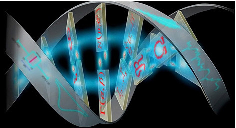
\includegraphics[height=1.5cm]{ggb_logo.pdf}}
\begin{document}
\maketitle
%%%%%%%%%%%%%%%%%%%%%%%%%%%%%%%%% SLIDE %%%%%%%%%%%%%%%%%%%%%%%%%%%%%%%%%
\begin{frame}{Table of contents}
  \setbeamertemplate{section in toc}[sections numbered]
  %\tableofcontents[hideallsubsections]
  \tableofcontents[]
\end{frame}
%%%%%%%%%%%%%%%%%%%%%%%%%%%%%%%%% SLIDE %%%%%%%%%%%%%%%%%%%%%%%%%%%%%%%%%
\section{Background}

\begin{frame}[fragile]{Gene Expression Signature Search (GESS)}

    \textcolor{blue}{Gene Expression Signatures (GES):}
    
    \footnotesize{Gene Expression Profiles \textcolor{blue}{(GEPs)} ($log_2$ ratios or z-scores) or Differentially Expressed Gene \textcolor{blue}{(DEG)} sets from disease or small molecule}
    \vspace{-0.2cm}
    \begin{itemize}
    \item Related transcriptional effects suggest related physiological effects on the cell 
    \item Used to \textcolor{blue}{uncover candidate drugs} to treat diseases, \textcolor{blue}{find connections} among small molecules
    \end{itemize}
    \vspace{-0.2cm}
    \begin{figure}
        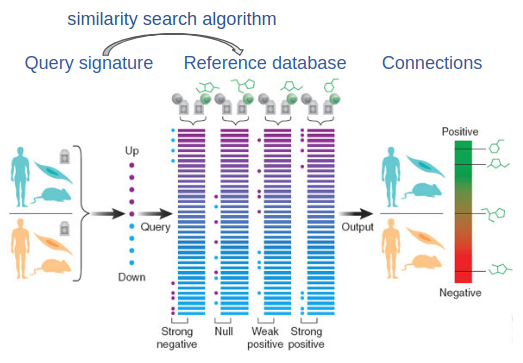
\includegraphics[width=7cm]{demo/images/gess_workflow.png}
    \end{figure}
    \begin{flushright} 
        \vspace{-0.5cm}
        \scriptsize{\textcolor{gray}{\cite{Lamb2006-du, Michnick2006-sr}}}
    \end{flushright} 
\end{frame}
%%%%%%%%%%%%%%%%%%%%%%%%%%%%%%%%%% SLIDE %%%%%%%%%%%%%%%%%%%%%%%%%%%%%%%%%
\begin{frame}{GES databases}
%    \centering
%    \begin{tabular}{ccc}
%      \toprule
%                   & CMap-Affy (original)   &   CMap-L1000 (new)\\
%      \midrule
%      Project      & CMap                    & CMap-LINCS\\
%      GESS algo.   & CMAP                    & CMAP-LINCS\\
%      Profiles     & 3,478                   & 473,647\\
%      \multirow{3}{*}{Perturbagens} & \multirow{3}{*}{Compounds: 1,309} & \multirow{3}{*}{Compounds: 19,811 \\ Gene knockdowns: $>$ 4k \\ 
%      Overexpression: $>$3k} \\
%      \bottomrule
%    \end{tabular}
\vspace{-0.2cm}
\begin{figure}
    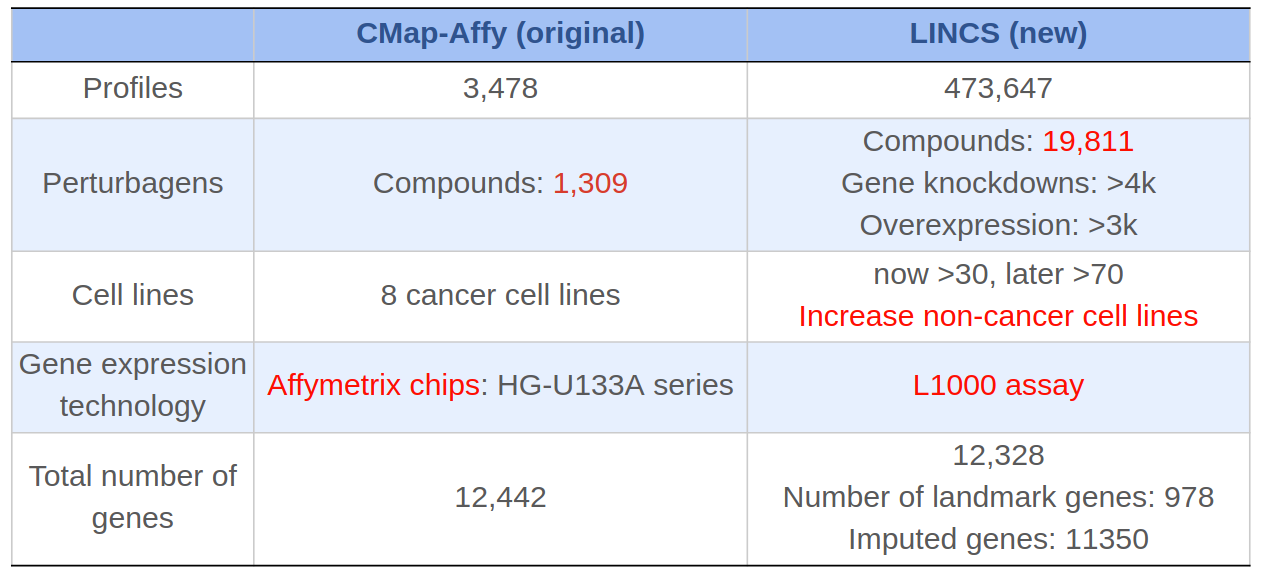
\includegraphics[width=11cm]{demo/images/ges_db.png}
\end{figure}
\end{frame}
%%%%%%%%%%%%%%%%%%%%%%%%%%%%%%%%% SLIDE %%%%%%%%%%%%%%%%%%%%%%%%%%%%%%%%%
\begin{frame}{Existing GESS algorithms}
  \begin{figure}
      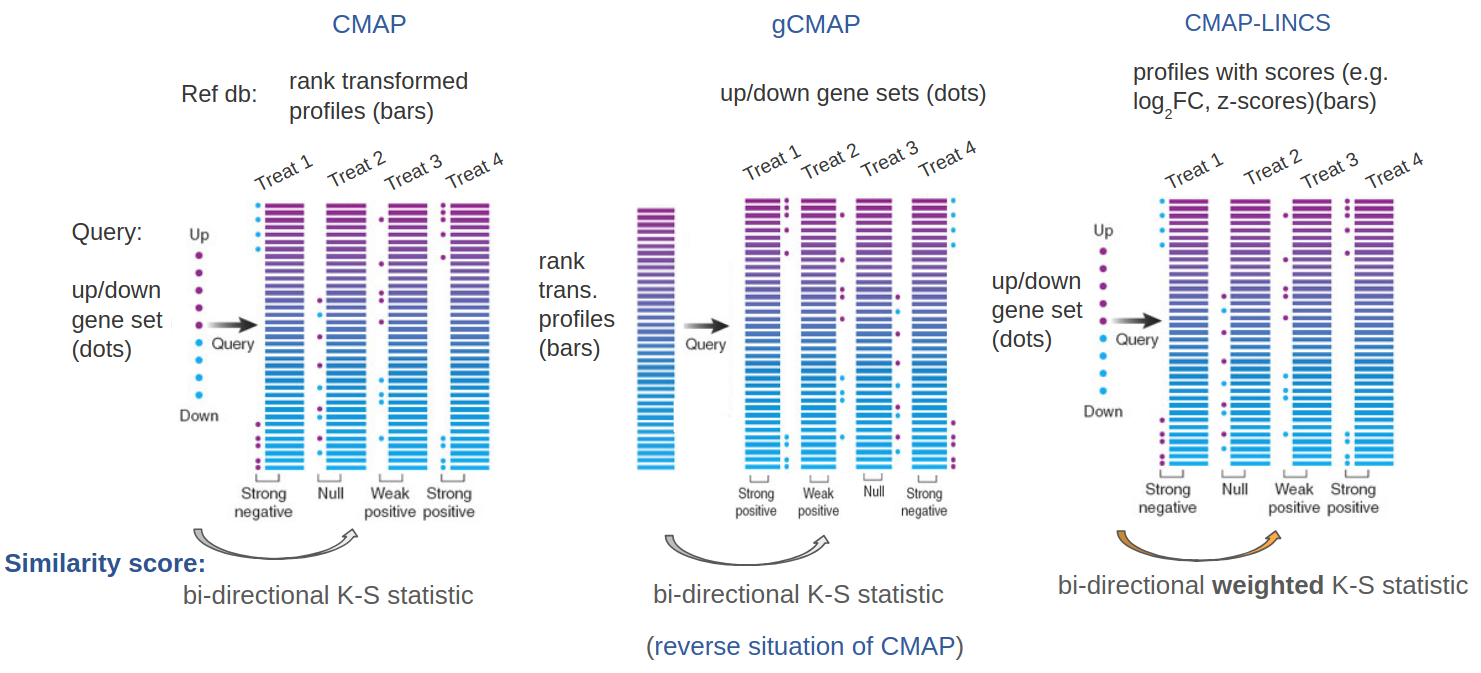
\includegraphics[width=12cm]{demo/images/gess_algo.png}
  \end{figure}
  \centering
  \scriptsize{\textcolor{gray}{\cite{Lamb2006-du, Pacini2013-or, Subramanian2017-fu}}}
\end{frame}
%%%%%%%%%%%%%%%%%%%%%%%%%%%%%%%%% SLIDE %%%%%%%%%%%%%%%%%%%%%%%%%%%%%%%%%
\begin{frame}{Existing GESS algorithms}
  \begin{figure}
      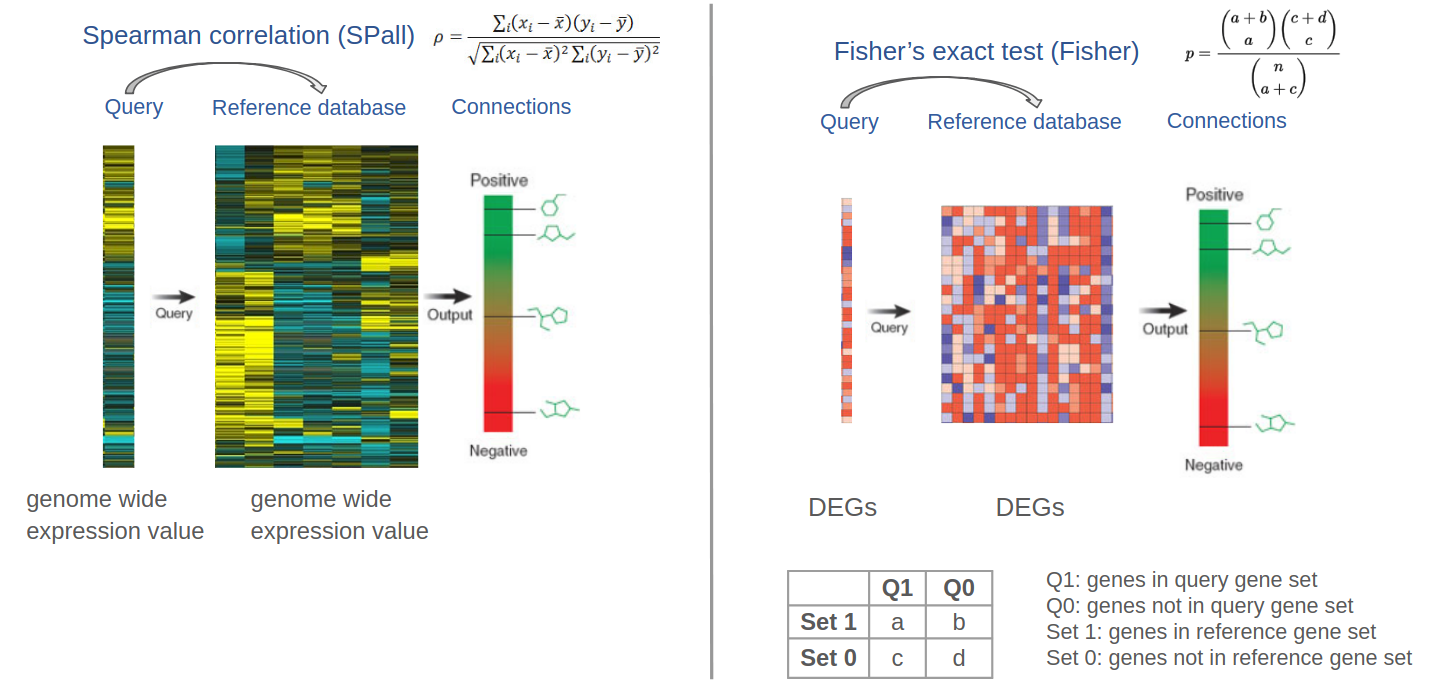
\includegraphics[width=12cm]{demo/images/sp_fisher.png}
  \end{figure}
\end{frame}
%%%%%%%%%%%%%%%%%%%%%%%%%%%%%%%%% SLIDE %%%%%%%%%%%%%%%%%%%%%%%%%%%%%%%%%
\begin{frame}{Comparison of existing GESS algorithms}
\vspace{-0.3cm}
  \begin{figure}
      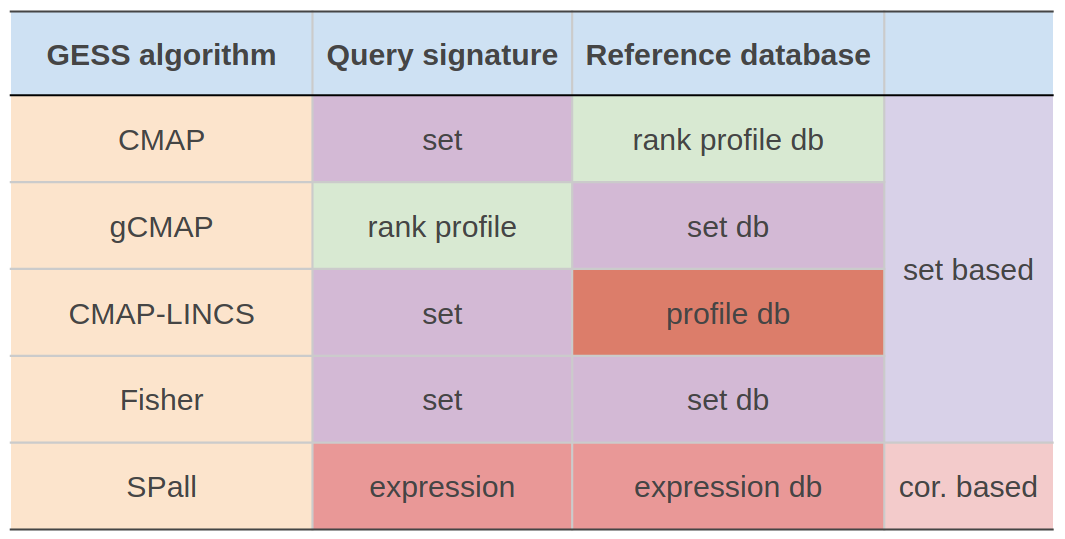
\includegraphics[width=9cm]{demo/images/cmp_gess.png}
  \end{figure}
\end{frame}
%%%%%%%%%%%%%%%%%%%%%%%%%%%%%%%%% SLIDE %%%%%%%%%%%%%%%%%%%%%%%%%%%%%%%%%
\section{Objectives and workplan}
%%%%%%%%%%%%%%%%%%%%%%%%%%%%%%%%% SLIDE %%%%%%%%%%%%%%%%%%%%%%%%%%%%%%%%%
\begin{frame}{Hypothesis with Workplan Objectives}
\vspace{-0.1cm}
    \begin{alertblock}{Hypothesis 1 (search methods):}
    	\begin{itemize}
            \item \alert{GESS methods can be optimized to predict the MOAs of experimental drugs and to identify new MOAs of known drugs for repurposing strategies}
    	\end{itemize}
    \end{alertblock}
    
    \begin{alertblock}{Hypothesis 2 (functional enrichment):}
    	\begin{itemize}
            \item \alert{Downstream functional enrichment analysis (FEA) will facilitate the interpretation of GESS results}
     	\end{itemize}
    \end{alertblock} 
     \begin{alertblock}{Hypothesis 3 (application):}
    \begin{itemize}
    \item \alert{A combined GESS and FEA workflow environment will facilitate the discovery of novel usages of known drugs and/or treatments of diseases (\textit{e.g.} healthy aging)}  
    \end{itemize}
        \end{alertblock} 
\end{frame}
%%%%%%%%%%%%%%%%%%%%%%%%%%%%%%%%% SLIDE %%%%%%%%%%%%%%%%%%%%%%%%%%%%%%%%%
\begin{frame}{Hypothesis with Workplan Objectives}
\vspace{-0.1cm}
    \begin{alertblock}{Hypothesis 1 (search methods):}
    	\begin{itemize}
            \item \alert{GESS methods can be optimized to predict the MOAs of experimental drugs and to identify new MOAs of known drugs for repurposing strategies}
            \begin{itemize}
                \item \textcolor{blue}{Implement GESS methods} (CMAP and CMAP-LINCS)
                \item \textcolor{blue}{Test performance of GESS methods} 
            \end{itemize}
    	\end{itemize}
    \end{alertblock}
    
    \begin{alertblock}{Hypothesis 2 (functional enrichment):}
    	\begin{itemize}
            \item \alert{Downstream functional enrichment analysis (FEA) will facilitate the interpretation of GESS results}
            \begin{itemize}
                \item \textcolor{blue}{Develop and implement FEA methods} 
                \item \textcolor{blue}{Test performance of FEA methods on GESS results}
                \item Enhance the FEA methods with \textcolor{blue}{drug-target network visualization}
                %\item Get enriched \textcolor{blue}{MOA categories} of top connected drugs in GESS result
            \end{itemize}
    	\end{itemize}
    \end{alertblock}    
\end{frame}


%%%%%%%%%%%%%%%%%%%%%%%%%%%%%%%%% SLIDE %%%%%%%%%%%%%%%%%%%%%%%%%%%%%%%%%
\begin{frame}{Hypothesis with Workplan Objectives}
\vspace{-1cm}
    \begin{alertblock}{Hypothesis 3 (application):}
    	\begin{itemize}
            \item \alert{A combined GESS and FEA workflow environment will facilitate the discovery of novel usages of known drugs and/or treatments of diseases (\textit{e.g.} healthy aging)}
            \begin{itemize}
                \item \textcolor{blue}{Implement permutation test} for the entire workflow to assess the robustness
                \item \textcolor{blue}{Apply} the entire workflow to a \textcolor{blue}{biological use case}
                \item \textcolor{blue}{Apply} the entire workflow to \textcolor{blue}{a series of} query signatures that are characteristic for \textcolor{blue}{healthy aging and longevity} in human
                \item \textcolor{blue}{Develop} the \textcolor{blue}{R/Bioconductor package \emph{signatureSearch}} to implement the GESS/FEA methods
            \end{itemize}
    	\end{itemize}
    \end{alertblock}
\end{frame}    
%%%%%%%%%%%%%%%%%%%%%%%%%%%%%%%%% SLIDE %%%%%%%%%%%%%%%%%%%%%%%%%%%%%%%%%
\begin{frame}{Workflow overview}
%\vspace{-0.3cm}
  \begin{figure}
      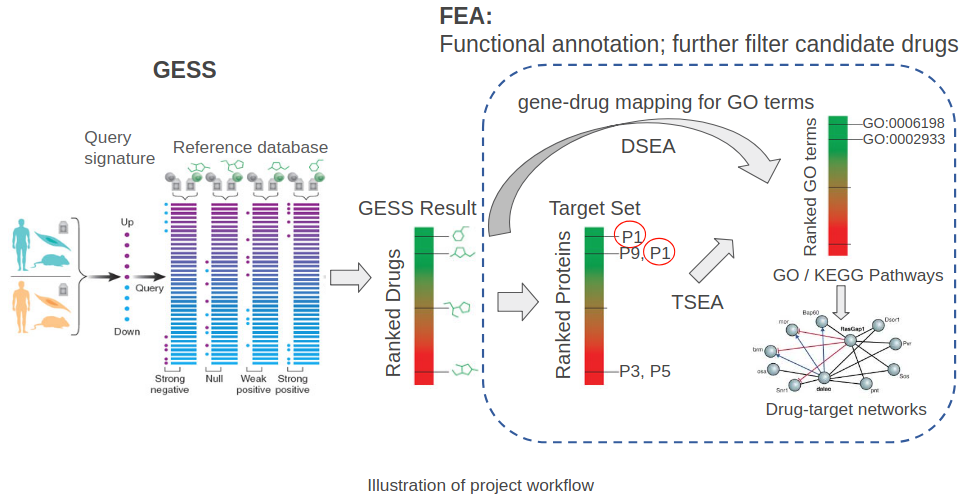
\includegraphics[width=12cm]{demo/images/workflow.png}
  \end{figure}
%\centering \scriptsize Illustration of project workflow
\end{frame}
%%%%%%%%%%%%%%%%%%%%%%%%%%%%%%%%% SLIDE %%%%%%%%%%%%%%%%%%%%%%%%%%%%%%%%%
\section{Methods}
\subsection{Signature Search algorithms}
%%%%%%%%%%%%%%%%%%%%%%%%%%%%%%%%% SLIDE %%%%%%%%%%%%%%%%%%%%%%%%%%%%%%%%%
\begin{frame}{Implementation of CMAP and CMAP-LINCS algorithms}
\vspace{-0.4cm}
    \begin{exampleblock}{CMap analysis options:}
    	\begin{itemize}
    	    \item \textcolor{green}{Online}
    	        \begin{itemize}
    	            \item \textcolor{blue}{Original CMAP website}, not updated
    	            \item \textcolor{blue}{CLUE website for CMAP-LINCS algo}, 2837/19,811 compounds in LINCS db
    	            \item \textcolor{blue}{L1000CDS\textsuperscript{2}}, 3924/19,811 compounds in LINCS db
    	        \end{itemize}
    	    \item \textcolor{green}{Local}
    	        \begin{itemize}
    	            \item \textcolor{blue}{DrugVsDisease}, not identical
    	            \item \textcolor{blue}{gCMAP}, switch around query and reference of CMAP algorithm.
    	            \item \textbf{\textcolor{blue}{No implementation for CMAP-LINCS algorithm.}}
    	        \end{itemize}
    	\end{itemize}
    \end{exampleblock}
\textcolor{green}{Local tools}: \textcolor{green}{limited access} but \textcolor{green}{crucial} to support large numbers of queries against any type of public/custom signature databases. \\
\alert{Implement CMAP and CMAP-LINCS algorithms in R}
\end{frame}
%%%%%%%%%%%%%%%%%%%%%%%%%%%%%%%%% SLIDE %%%%%%%%%%%%%%%%%%%%%%%%%%%%%%%%%
\begin{frame}{Performance testing of GESS methods}
    \textcolor{blue}{Recall test}\\
        \begin{itemize}
            \item Do drugs with \textcolor{blue}{similar molecular effects} or \textcolor{blue}{target sites} cluster together?
            \item Various drug classifications (MOA) can be used to test systematically
        \end{itemize}
    \textcolor{blue}{Test Schema}\\
        \begin{itemize}
            \item \textcolor{blue}{Categorize} compounds according to \textcolor{blue}{MOA} and \textcolor{blue}{target} information
            \item \textcolor{blue}{Database:} LINCS
        \end{itemize}
    \begin{figure}
        \centering
        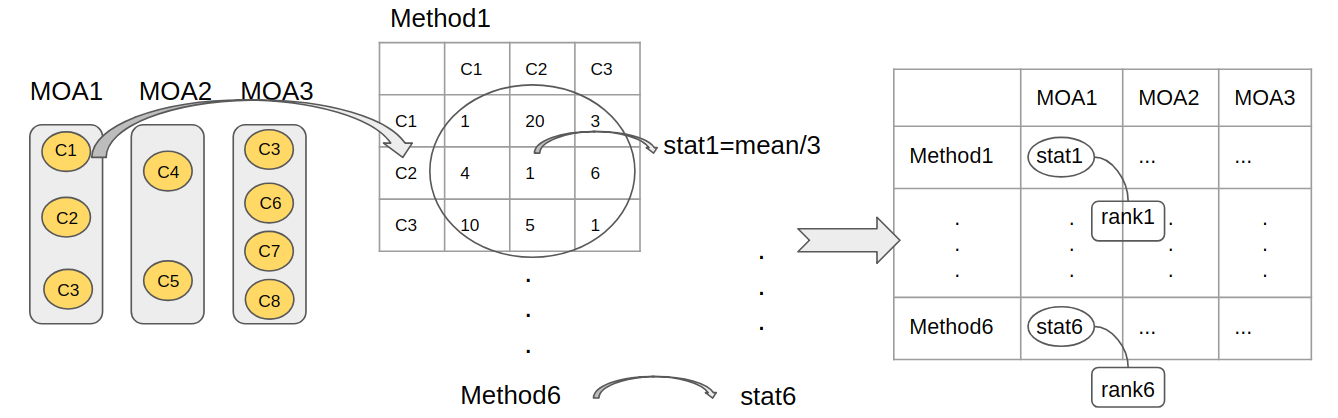
\includegraphics[width=10.5cm]{demo/images/test_gess.png}
    \end{figure}
\end{frame}
\subsection{Functional Enrichment Methods}
%%%%%%%%%%%%%%%%%%%%%%%%%%%%%%%%% SLIDE %%%%%%%%%%%%%%%%%%%%%%%%%%%%%%%%%
\begin{frame}{Methods to functionally annotate GESS results (FEA)}
  \vspace{-0.3cm}
  \begin{figure}
      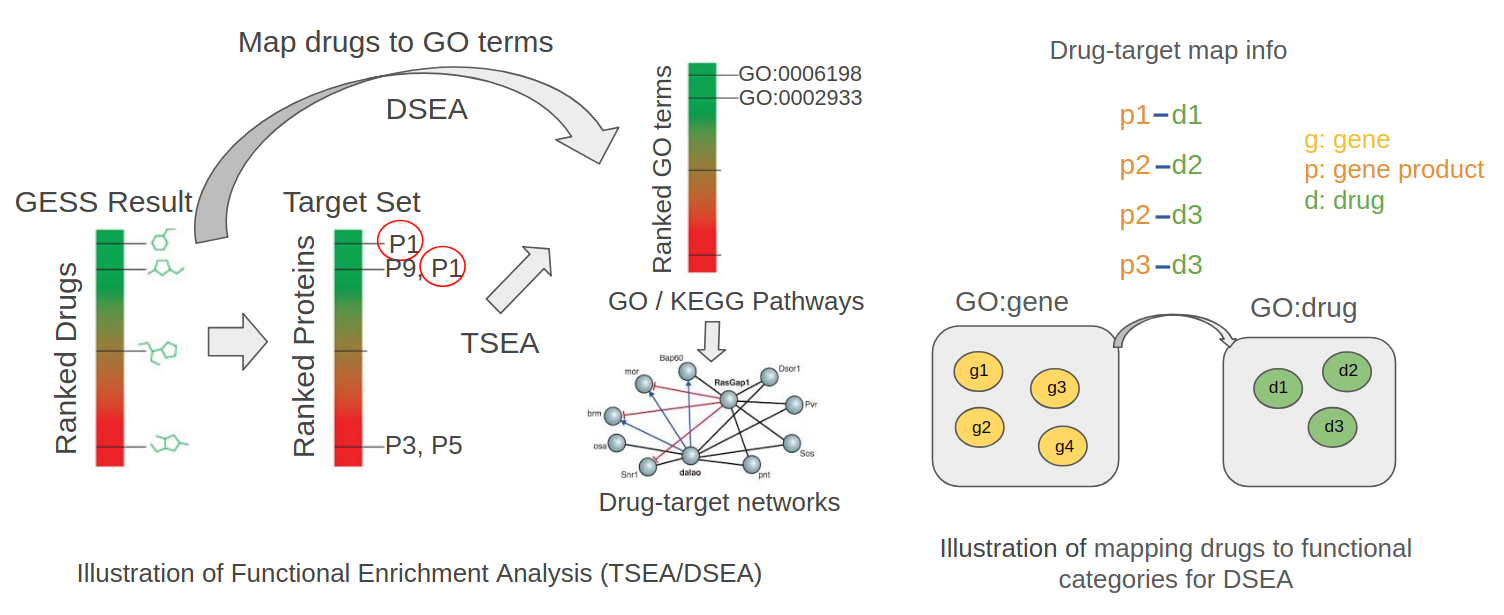
\includegraphics[width=11cm]{demo/images/fea_illu.png}
  \end{figure}
  \vspace{-0.8cm}
  \small
   \begin{columns}[T,onlytextwidth]
    \column{0.5\textwidth}
      \begin{alertblock}{\small Target Set Enrichment Analysis (TSEA)}
        \vspace{-0.2cm}
        \begin{itemize} \itemsep0pt
            \item \textcolor{blue}{Get targets} of top connected drugs
            \item \alert{Requirement:} Support target set with duplications. 
            \item 3 enrichment methods \alert{on targets} that weight duplications
        \end{itemize}
      \end{alertblock}
    \column{0.5\textwidth}
      \begin{alertblock}{\small Drug Set Enrichment Analysis (DSEA)}
        \vspace{-0.2cm}
        \begin{itemize}
            \item \textcolor{blue}{Map drugs} to functional categories (GO/KEGG) via drug-target information. 
            \item 2 enrichment methods \alert{on drugs}, overcome the duplication problem.
        \end{itemize}
      \end{alertblock}
  \end{columns}
\end{frame}
%%%%%%%%%%%%%%%%%%%%%%%%%%%%%%%%% SLIDE %%%%%%%%%%%%%%%%%%%%%%%%%%%%%%%%%
\begin{frame}{Drug Annotation Databases}
\vspace{0.3cm}
  \begin{columns}[T,onlytextwidth]
    \column{0.6\textwidth}
        \small
        \textcolor{blue}{DrugBank}: \textcolor{blue}{11,002} drug entries \\
        \vspace{0.1cm}
        \textcolor{blue}{Touchstone:} \\
        Part of LINCS database \\
        Well-annotated \textcolor{blue}{2837} compounds \\
        \vspace{0.1cm}
        \textcolor{blue}{STITCH:} 
        \vspace{-0.3cm}
        \begin{figure}
          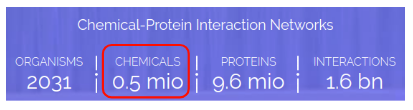
\includegraphics[width=6cm]{demo/images/sti.png}
        \end{figure}
        \vspace{-0.5cm}
        \begin{itemize} \itemsep0pt
            \item Get combined drug-target information 
            \item Exclude drugs with more than 100 targets 
            \item Exclude targets with more than 100 drugs
            \item \textcolor{blue}{Target space:} all targets after exclusion (5682)
            \item \textcolor{blue}{Drug space:} all drugs after exclusion (22481)
        \end{itemize}

    \column{0.4\textwidth}
    \vspace{-0.6cm}
      \begin{figure}
        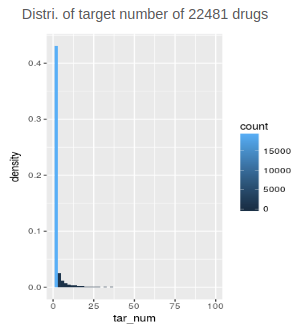
\includegraphics[width=3.5cm, height=3.8cm]{demo/images/distri1.png} \\
        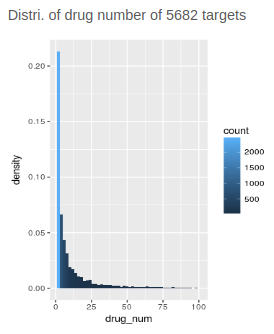
\includegraphics[width=3.5cm, height=3.8cm]{demo/images/distri2.png}
      \end{figure}
  \end{columns}
\end{frame}
%%%%%%%%%%%%%%%%%%%%%%%%%%%%%%%%% SLIDE %%%%%%%%%%%%%%%%%%%%%%%%%%%%%%%%%
\begin{frame}{TSEA}
\vspace{-0.8cm}
\alert{\textbf{a. Duplication adjusted hypergeometric test (dup\_hyperG})}
\begin{itemize}
    \item \alert{Important modification:} support target set with duplications
    \item \textcolor{blue}{Input:} targets of top ranked drugs in GESS result
\end{itemize}
hypergeometric test (only support unique gene/protein set):\\
\vspace{0.5cm}
\begin{columns}
    \column{0.3\textwidth}
        \begin{equation}
           \displaystyle p=\sum_{k=x}^{n}\frac {{D \choose k}{{N-D} \choose {n-k}}}{{N \choose n}}
        \end{equation}
    \column{0.58\textwidth}
      \scriptsize
      \textcolor{blue}{$N$}: total number of genes/proteins contained in the entire annotation (universe) \\
      \textcolor{blue}{$D$}:  number of genes annotated at a specific GO node \\
      \textcolor{blue}{$n$}: total number
of genes in the test set \\
      \textcolor{blue}{$x$}: number of genes in the test set annotated at a specific GO node
\end{columns}
\vspace{0.4cm}
Values of \textcolor{blue}{$n$}, \textcolor{blue}{$x$} are adjusted by frequency of target proteins in the test set
\end{frame}
%%%%%%%%%%%%%%%%%%%%%%%%%%%%%%%%% SLIDE %%%%%%%%%%%%%%%%%%%%%%%%%%%%%%%%%
\begin{frame}{TSEA}
\alert{\textbf{b. Modified GSEA (m\_GSEA)}}
\small
\begin{exampleblock}{Introduction to Gene Set Enrichment Analysis (GSEA)}
    \textcolor{green}{Input:} ranked gene list $L = \{g_1,...,g_N\}$ with score $\{r_1,...,r_N\}$ \\
     a priori defined gene set $S$ (genes in a KEGG pathway or GO category) \\
    \textcolor{green}{Goal:} determine whether $S$ randomly distributed throughout $L$ or \textcolor{green}{primarily found at the top or bottom}. \\
\end{exampleblock}
\vspace{-0.1cm}
\begin{columns}
    \column{0.3\textwidth}
        \begin{figure}
            \centering
            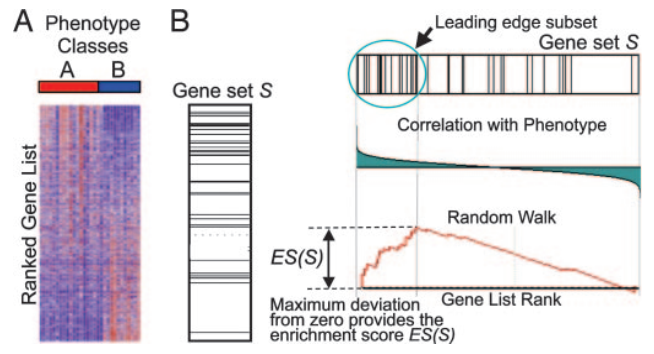
\includegraphics[width=4.8cm]{demo/images/gsea.png}
            \label{fig:gsea}
        \end{figure}
        \scriptsize{\textcolor{gray}{\cite{Subramanian2005-ro}}}
    \column{0.59\textwidth}
        \renewcommand*{\normalfont}{\relax}
        \scriptsize
        \begin{align}
        &\scriptstyle P_{hit}(S,i)=\sum_{g_j\in S, j\leq i}\frac{|r_j|^p}{N_R}, \mathrm{where}\ N_R=\sum_{g_j\in S} {|r_j|^p} 
        \label{eq:nr}\\
        &\scriptstyle P_{miss}(S,i)=\sum_{g_j\notin S, j\leq i}\frac{1}{(N-N_H)} \\
        &\scriptstyle ES = \mathrm{maximum\  deviation\  from\  zero\  of\  } P_{hit} - P_{miss}
        \end{align}
      
      \hspace{1cm}\scriptsize{\textcolor{green}{$r_j$}\textcolor{gray}{: score of gene $j$ in $L$;} \textcolor{green}{$N$}\textcolor{gray}{: number of genes in $L$;} \\ 
      \hspace{1cm}\textcolor{green}{$N_H$} \textcolor{gray}{: number of genes in $S$}} \\
      \vspace{0.2cm}
      \footnotesize
      \hspace{0.65cm}\textcolor{green}{$p=0$}: $ES$: \textcolor{green}{standard Kolmogorov–Smirnov statistic} \\
      \begin{itemize} \itemsep0pt
          \item[\textcolor{green}{$\checkmark$}]  \textcolor{green}{$p=1$}: $ES$: \textcolor{green}{weighted K-S like statistic}
      \end{itemize}
      
\end{columns}
\vspace{0.4cm}
\end{frame}
%%%%%%%%%%%%%%%%%%%%%%%%%%%%%%%%% SLIDE %%%%%%%%%%%%%%%%%%%%%%%%%%%%%%%%%
\begin{frame}{TSEA}
    \begin{alertblock}{b. m\_GSEA}
        \begin{itemize}
            \item \textcolor{blue}{Input:} scored ranked target list $L_{tar}$ of all genes/proteins in universe
            \item How to convert target set with duplications to $L_{tar}$?
        \end{itemize}
        \vspace{-0.5cm}
        \begin{figure}
            \centering
            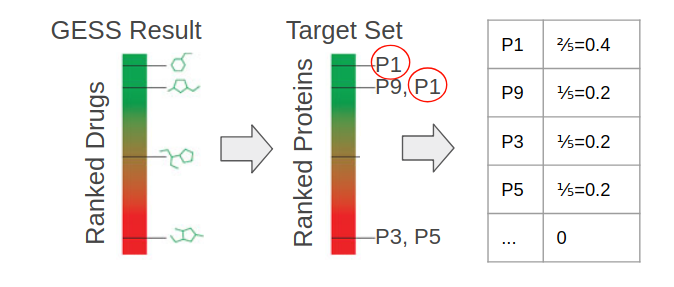
\includegraphics[width=8cm]{demo/images/m_gsea.png}
        \end{figure}
        \vspace{-0.5cm}
        \begin{itemize}
            \begin{itemize}
                \item For proteins in target set, set $N_{dup}/N_{total\_tar}$ as their scores
                    \begin{itemize}
                        \item $N_{dup}$: number of duplication of a protein
                        \item $N_{total\_tar}$: total number of proteins in target set
                    \end{itemize}
                \item For proteins in universe, but not in target set, set scores as 0
            \end{itemize}
        \end{itemize}
    \end{alertblock}
\end{frame}
%%%%%%%%%%%%%%%%%%%%%%%%%%%%%%%%% SLIDE %%%%%%%%%%%%%%%%%%%%%%%%%%%%%%%%%
\begin{frame}{TSEA}
  \vspace{-0.55cm}
    \begin{alertblock}{b. m\_GSEA}
        \begin{itemize}
            \item \alert{GSEA modification}
              \begin{itemize}
                \item Why it is needed? \\
                     \alert{large portion of zero exists} in scores of $L_{tar}$
                \item If scores of genes in $S$ are all zeros, set $ES(S)$ as -1
                \item If part of scores of genes in $S$ are zero, set \resizebox{0.33\hsize}{!}{$\displaystyle N_R=\sum_{g_j\in S}|r_j|^p+0.002*\sum_{g_j\in S}I_{r_j=0}$}, \\ refer to equation \ref{eq:nr}
                    \begin{itemize}
                        \small \item \textcolor{blue}{Reason:} decrease the weight of genes in $S$ that have non-zero scores \\
%                        \begin{equation}
%                            \resizebox{0.45\hsize}{!}{
%                            \displaystyle P_{hit}(S,i)=\sum_{g_j\in S, j\leq i}\frac{|r_j|^p}{N_R}, \mathrm{where}\ N_R=\sum_{g_j\in S} {|r_j|^p}}
%                        \end{equation}
%                        \begin{center}
%                            $r_j$: score of gene $j$ in $L$
%                        \end{center}
                    \end{itemize}
                \item Set largest number of $P_{hit}  - P_{miss}$ as $ES$
                    \begin{itemize}
                        \small \item \textcolor{blue}{Reason:} only want to find gene set $S$ enriched at the top of $L_{tar}$
                    \end{itemize}
            \end{itemize}
        \end{itemize}
    \end{alertblock}
\end{frame}
%%%%%%%%%%%%%%%%%%%%%%%%%%%%%%%%% SLIDE %%%%%%%%%%%%%%%%%%%%%%%%%%%%%%%%%
\begin{frame}{TSEA}
    \begin{alertblock}{c. meanAbs (mabs)}
        \footnotesize
        \begin{itemize}
            \item \itemsep0pt \textcolor{blue}{Input:} Scored ranked target list $L_{tar}$
            \item \itemsep0pt \textcolor{blue}{Calculation of $mabs$ score:} \\
            Given a priori defined gene set $S$ (genes in a KEGG pathway or GO category)
            \renewcommand*{\normalfont}{\relax}
            \scriptsize
            \begin{equation}
                \resizebox{0.25\hsize}{!}{
                \scriptstyle mabs(S)=\frac{1}{K}\sum_{i=1}^{K}|T_i|}
            \end{equation}
            \begin{center}
                \textcolor{blue}{$T_i$}: score of gene $i$ in $S$; \textcolor{blue}{$K$}: number of genes in $S$ 
            \end{center}
            \footnotesize
            \item \itemsep0pt \textcolor{blue}{Calculation of normalized $mabs$ score $(Nmabs)$:} \\
            \textcolor{blue}{Adjust for variation of gene set size.} For each $S$, make 1000 time of random permutation of $L_{tar}$ and determine $mabs(S,\pi)$.
            \renewcommand*{\normalfont}{\relax}
            \scriptsize

            \begin{equation}
                \resizebox{0.4\hsize}{!}{
                \scriptstyle
                Nmabs(S)=\frac{mabs(S)-\mathrm{median}(mabs(S,\pi))}{\mathrm{sd}(mabs(S,\pi))}}
            \end{equation}
            
            \footnotesize
            \item \itemsep0pt \textcolor{blue}{Estimate nominal $p$ value} \\
            portion of $mabs(S,\pi)$ greater than $mabs(S)$
            \item \itemsep0pt \textcolor{blue}{Multiple Hypothesis Testing} \\
            $p$ values are adjusted by Benjamini-Hochberg method
        \end{itemize}
      \hfill \scriptsize{\textcolor{gray}{\cite{Fang2012-ms}}}
    \end{alertblock}
\end{frame}
%%%%%%%%%%%%%%%%%%%%%%%%%%%%%%%%% SLIDE %%%%%%%%%%%%%%%%%%%%%%%%%%%%%%%%%
\begin{frame}{DSEA}
  \vspace{-0.5cm}
    \textcolor{blue}{Functional database:} drug-to-functional category mappings \\
    \textcolor{blue}{Query:} directly be \textcolor{blue}{drugs} \\
    \vspace{0.2cm}
    \begin{alertblock}{a. hypergeometric test (hyperG)}
        \begin{itemize}
            \item \textcolor{blue}{Input:} top ranked drugs in GESS result
        \end{itemize}
    \end{alertblock}
    \begin{alertblock}{b. GSEA}
        \begin{itemize}
            \item \textcolor{blue}{Input:} ranked drug list of all drugs in GESS result
            \item What score is appropriate for this drug list?
            \begin{itemize}
                \item Similarity scores in GESS result. \\
            \end{itemize}
        \end{itemize}
    \end{alertblock}
\end{frame}
%%%%%%%%%%%%%%%%%%%%%%%%%%%%%%%%% SLIDE %%%%%%%%%%%%%%%%%%%%%%%%%%%%%%%%%
\begin{frame}{Summary of methods implementation}
\vspace{-0.5cm}
  \begin{figure}
      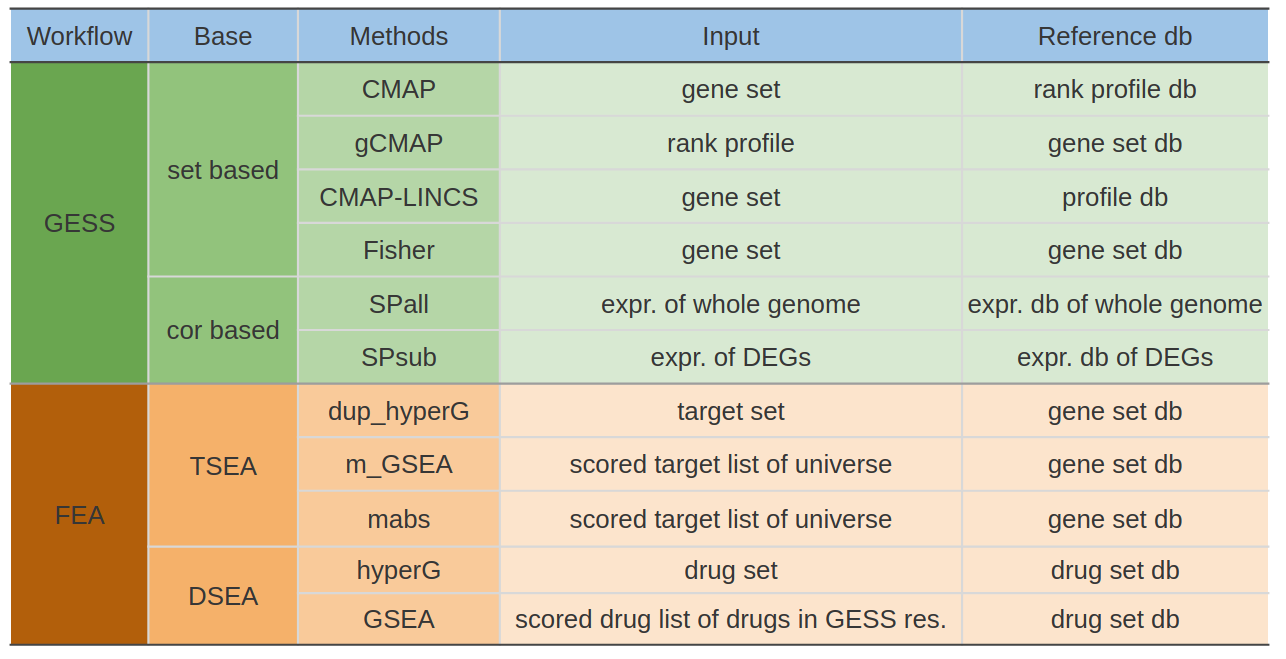
\includegraphics[width=10.2cm]{demo/images/sum_imple.png}
  \end{figure}
\end{frame}

\subsection{Performance tests}
%%%%%%%%%%%%%%%%%%%%%%%%%%%%%%%%% SLIDE %%%%%%%%%%%%%%%%%%%%%%%%%%%%%%%%%
\section{Results}
%%%%%%%%%%%%%%%%%%%%%%%%%%%%%%%%% SLIDE %%%%%%%%%%%%%%%%%%%%%%%%%%%%%%%%%
\begin{frame}{Performance testing of GESS methods}
\vspace{-0.25cm}
    \begin{figure}
        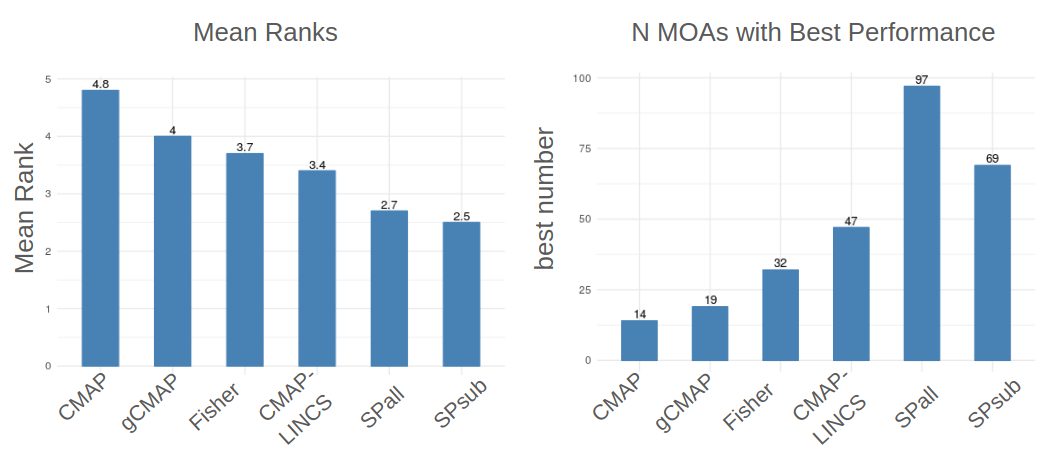
\includegraphics[width=10cm]{demo/images/gess_test.png}
    \end{figure}
    \vspace{-0.6cm}
    \textcolor{blue}{Conclusion:}\\
    \begin{itemize}
        \item \textcolor{blue}{Correlation} based methods perform better than set enrichment
        \item \textcolor{blue}{CMAP-LINCS} performs best among set enrichment methods
        \item \textcolor{blue}{Choice depends on type of query and reference database}
    \end{itemize}
\end{frame}
%%%%%%%%%%%%%%%%%%%%%%%%%%%%%%%%% SLIDE %%%%%%%%%%%%%%%%%%%%%%%%%%%%%%%%%
\begin{frame}{Performance testing of FEA methods on GESS results}
\vspace{-3cm}
    \begin{itemize}
        \item Robustness of \textcolor{blue}{hyperG} and \textcolor{blue}{GSEA} tested \textcolor{blue}{individually}
        \item \textcolor{blue}{Robust} performance of each method
            \begin{itemize}
                \item \textcolor{blue}{Support:} 5\%, 10\%, 15\% randomized GO categories can be significantly recalled
            \end{itemize}
        \item \textcolor{blue}{Direct performance comparison} among FEA methods is \textcolor{blue}{absent}. In future plan
    \end{itemize}
\end{frame}
%%%%%%%%%%%%%%%%%%%%%%%%%%%%%%%%% SLIDE %%%%%%%%%%%%%%%%%%%%%%%%%%%%%%%%%
\begin{frame}{Biological application of the entire workflow}
\vspace{-0.1cm}
    \begin{itemize}
        \footnotesize
        \item \textcolor{blue}{Query signature:} human longevity related DEGs from \cite{Peters2015-vg}
        \item \textcolor{blue}{Reference database:} LINCS
        \item \textcolor{blue}{Goal:} find Longevity Associated Drugs (LADs). 
        \item \textcolor{blue}{Method:} CMAP-LINCS for GESS, FEA: functional annotation and further filter
    \end{itemize}
\vspace{-0.1cm}
\begin{columns}
\column{0.66\textwidth}
    \begin{table}
    \small
    \resizebox{0.99\hsize}{!}{
    \begin{tabular}{ccccccc}
  \hline
 Rank & Pert & Type & NCS & Tau & NCSct & Ref. \\ 
  \hline
 1 & BRD-K63954456 & NEU & 1.92 & 99.95 & 0.31 &  \\ 
 2 & SB-205384 & A549 & -1.73 & -99.95 & -1.02 &  \\ 
 3 & clioquinol & PC3 & -1.82 & -99.95 & -0.66 &  \\ 
 4 & BRD-K01006500 & PC3n & -1.75 & -99.95 & -1.11 &  \\ 
 5 & BRD-K62841356 & VCAP & -1.65 & -99.93 & -1.65 &  \\ 
 6 & BRD-K31844452 & VCAP & -1.78 & -99.93 & -1.19 &  \\ 
 7 & BRD-K12411950 & MCF7 & 1.71 & 99.91 & 0.9 &  \\ 
 8 & embelin & VCAP & -1.66 & -99.91 & 0.82 &  \\ 
 72 & gsk-1070916 & PHH & 1.49 & 99.55 & -0.31 &  \\ 
 185 & pitavastatin & VCAP & 1.58 & 98.98 & 1.27 &  \\ 
 230 & calcitriol & SKB & 1.64 & 98.84 & 1.12 &  \\ 
 266 & irinotecan & VCAP & 1.56 & 98.67 & 0.9 &  \\ 
 267 & alitretinoin & NEU & 1.41 & 98.66 & -0.89 &  \\ 
 \rowcolor{red!72}  270 & caffeine & HA1E & 1.36 & 98.66 & 0.78 & \citep{Bridi2015-hs} \\ 
 303 & gemfibrozil & VCAP & 1.39 & 98.49 & 0.86 &  \\ 
 \rowcolor{yellow!70}  304 & sirolimus & FIBRE NPC & 1.44 & 98.49 & 0 & \citep{Ehninger2014-ip} \\ 
 \rowcolor{yellow!70}  325 & indirubin & HA1E & -1.4 & -98.39 & -0.02 & \citep{Spindler2012-an} \\ 
 \rowcolor{yellow!70}  377 & alpha-estradiol & A375 & -1.30 & -98.17 & -1.02 & \citep{Harrison2014-yo} \\
 \rowcolor{yellow!70} 469 & phenformin & NEU & 1.45 & 97.73 & -0.79 & \citep{Cabreiro2013-zc} \\ 
 ... & ... & ... & ... & ... & ... &  \\ 
   \hline
\end{tabular}}
  \end{table}
\column{0.25\textwidth}
\scriptsize
Top 8 connected drugs, drugs filtered after FEA, and \textcolor{yellow!70}{\textbf{known LADs}} in the GESS result. \\
\addlinespace
\textcolor{red!70}{\textbf{known LADs that are also found after FEA}}.
    \end{columns}
\end{frame}
%%%%%%%%%%%%%%%%%%%%%%%%%%%%%%%%% SLIDE %%%%%%%%%%%%%%%%%%%%%%%%%%%%%%%%%
\begin{frame}{Biological application of the entire workflow}
\vspace{-0.5cm}
\begin{columns}
\column{0.45\textwidth}
    \begin{figure}
        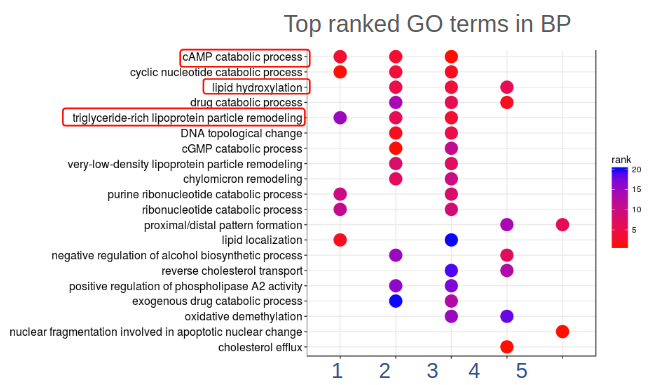
\includegraphics[width=6.3cm]{demo/images/top_go_bp.png}\\
        \vspace{0.2cm}
        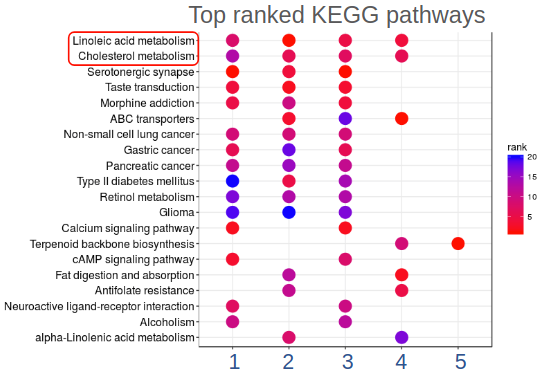
\includegraphics[width=5.2cm]{demo/images/top_kegg.png}
    \end{figure}
\column{0.5\textwidth}
    \vspace{-0.5cm}
    \begin{figure}
        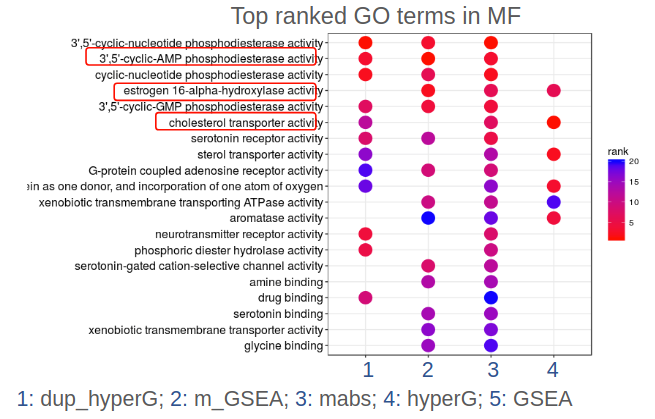
\includegraphics[width=6.3cm]{demo/images/top_go_mf.png}
    \end{figure}
    \small
    \textcolor{blue}{cAMP catabolic process}, \textcolor{blue}{lipid hydroxylation}, \textcolor{blue}{lipoprotein particle remodeling} are enriched, may associate with human longevity. \\
    \addlinespace
    \textcolor{blue}{Good agreements} for GO terms in \textcolor{blue}{BP}, \textcolor{blue}{MF} ontology and \textcolor{blue}{KEGG} pathways
\end{columns}
\end{frame}
%%%%%%%%%%%%%%%%%%%%%%%%%%%%%%%%% SLIDE %%%%%%%%%%%%%%%%%%%%%%%%%%%%%%%%%
\begin{frame}{Construction of drug-target networks}
\vspace{-0.5cm}
\begin{columns}
\footnotesize
\column{0.28\textwidth}
    \begin{figure}[t]
        \begin{flushleft}
        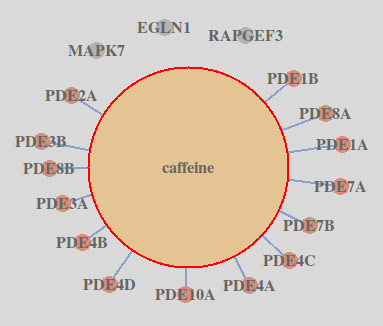
\includegraphics[width=3.2cm]{demo/images/dtnet_camp.png}
        \end{flushleft}
    \end{figure}
    
    GO:0006198 (\textcolor{blue}{cAMP catabolic process})
    \begin{itemize}
        \item \textcolor{blue}{Assumption:} caffeine may affect human longevity.
        \item \textcolor{blue}{positively connected} with chronological age status
    \end{itemize}
    
\column{0.36\textwidth}
\vspace{0.2cm}
    \begin{figure}[t]
        \begin{flushleft}
        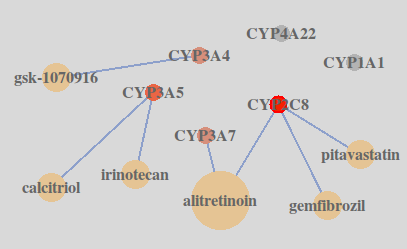
\includegraphics[width=3.8cm]{demo/images/dtnet_hydroxy.png}
        \end{flushleft}
    \end{figure}
    \vspace{0.3cm}
    GO:0002933 (\textcolor{blue}{lipid hydroxylation})
    \begin{itemize}
        \item calcitriol, irinotecan, alitretinoin, gemfibrozil, pitavastatin, and gsk-1070916 could affect lipid hydroxylation. 
        \item \textcolor{blue}{Assumption:} candidate LADs
    \end{itemize}
\column{0.28\textwidth}
    \vspace{-0.9cm}
        \begin{figure}[t]
            \begin{flushleft}
                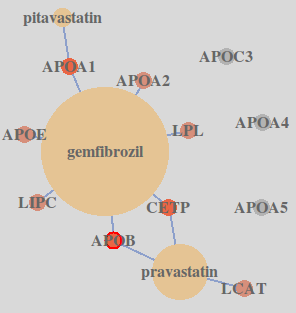
\includegraphics[width=2.8cm]{demo/images/dtnet_remodel.png}
            \end{flushleft}
        \end{figure}

    GO:0034370  (\textcolor{blue}{triglyceride-rich lipoprotein particle remodeling})
    \begin{itemize}
        \item gemfibrozil, pitavastatin also found. 
    \end{itemize}
\end{columns}
\end{frame}
%%%%%%%%%%%%%%%%%%%%%%%%%%%%%%%%% SLIDE %%%%%%%%%%%%%%%%%%%%%%%%%%%%%%%%%
\section{Future plans}
%%%%%%%%%%%%%%%%%%%%%%%%%%%%%%%%% SLIDE %%%%%%%%%%%%%%%%%%%%%%%%%%%%%%%%%
\begin{frame}{Overview of workplans}
\vspace{-0.3cm}
  \begin{itemize}
    \item[{$\checkmark$}] Implement GESS methods (CMAP and CMAP-LINCS)
    \item[{$\checkmark$}] Test performance of GESS methods
    \item[{$\checkmark$}] Develop and implement FEA methods
    \item[\textcolor{red}{$\bigstar$}] \textcolor{red}{Test performance of FEA methods on GESS results}
    \item[{$\checkmark$}] Construct drug-target networks for visualization
    \item[{$\checkmark$}] Apply the entire workflow to a biological use case.
    \item[\textcolor{red}{$\bigstar$}] \textcolor{red}{Use MOA annotations to do DSEA on GESS results}
    \item[\textcolor{red}{$\bigstar$}] \textcolor{red}{Implement permutation test for the entire workflow to assess the robustness}
    \item[\textcolor{red}{$\bigstar$}] \textcolor{red}{Apply the entire workflow to a series of query signatures that are characteristic for healthy aging and longevity in human}
    \item[\textcolor{red}{$\bigstar$}] \textcolor{red}{Develop the R/Bioconductor package \emph{signatureSearch} to implement the GESS/FEA methods}
  \end{itemize}
\end{frame}
%%%%%%%%%%%%%%%%%%%%%%%%%%%%%%%%% SLIDE %%%%%%%%%%%%%%%%%%%%%%%%%%%%%%%%%
\begin{frame}{Performance testing of FEA methods on GESS results}
\vspace{-0.4cm}
\textcolor{blue}{Benchmark datasets:} \\
34 disease gene expression datasets whose \textcolor{blue}{target pathways are known} in KEGG \textcolor{gray}{\cite{Dong2016-ve}} \\
\vspace{0.2cm}
\textcolor{blue}{Methods:} \\
\begin{itemize}
    \item GESs of the disease datasets will be used for GESSs against the LINCS database.
    \item The resulting ranked drug lists will be subjected to the FEA methods to see whether the target KEGG pathways could be enriched
\end{itemize}
\textcolor{blue}{Evaluate the performance:} \\ \textcolor{blue}{Sensitivity}, \textcolor{blue}{Prioritization}, and \textcolor{blue}{False Positive Rate}. \textcolor{gray}{\cite{Tarca2013-lv}} 
\end{frame}
%%%%%%%%%%%%%%%%%%%%%%%%%%%%%%%%% SLIDE %%%%%%%%%%%%%%%%%%%%%%%%%%%%%%%%%
\begin{frame}{Permutation test to determine the workflow robustness}
\vspace{-1cm}
    \begin{figure}
        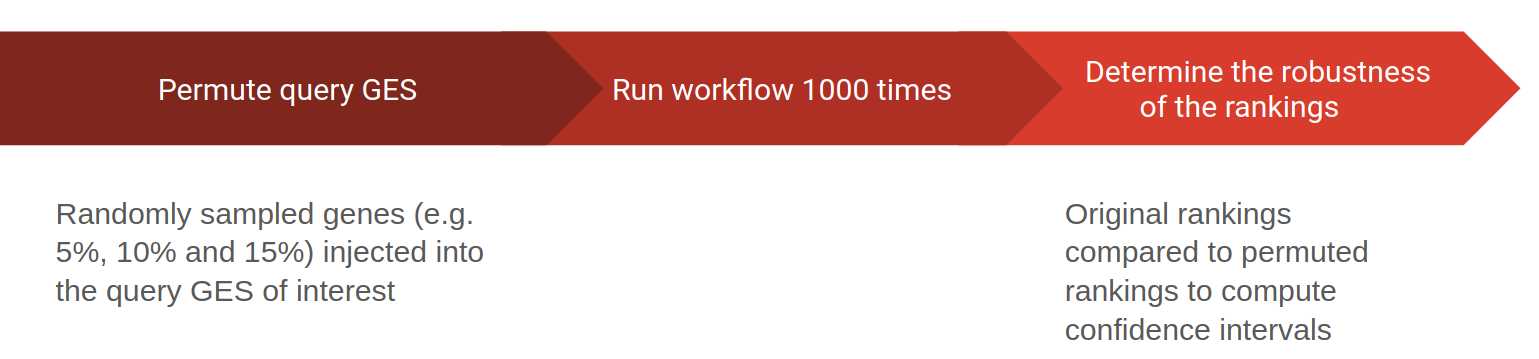
\includegraphics[width=12cm]{demo/images/perm_wkfl.png}
    \end{figure}
    \textcolor{blue}{Permutation test:}\\
The confidence intervals of drug/pathway rankings expressing the robustness of the rankings \\
\end{frame}
%%%%%%%%%%%%%%%%%%%%%%%%%%%%%%%%% SLIDE %%%%%%%%%%%%%%%%%%%%%%%%%%%%%%%%%
\section{Other projects}
%%%%%%%%%%%%%%%%%%%%%%%%%%%%%%%%% SLIDE %%%%%%%%%%%%%%%%%%%%%%%%%%%%%%%%%
\begin{frame}{DrugbankR package}
\vspace{-1.6cm}
\textcolor{blue}{Motivation:} \\
    \begin{itemize}
        \item no Application Programming Interface on DrugBank website
        \item No local tools to get drug annotations in batch.
    \end{itemize}
\vspace{0.6cm}
\textcolor{blue}{Utility:} \\
Query drug-target annotations in DrugBank database through R. 
\end{frame}
%%%%%%%%%%%%%%%%%%%%%%%%%%%%%%%%% SLIDE %%%%%%%%%%%%%%%%%%%%%%%%%%%%%%%%%
\begin{frame}{Drug-target web service implemented in Shiny}
\vspace{-0.6cm}
\textcolor{blue}{\href{https://tgirke.shinyapps.io/geneTargetAnno/}{https://tgirke.shinyapps.io/geneTargetAnno/}}
    \begin{figure}
        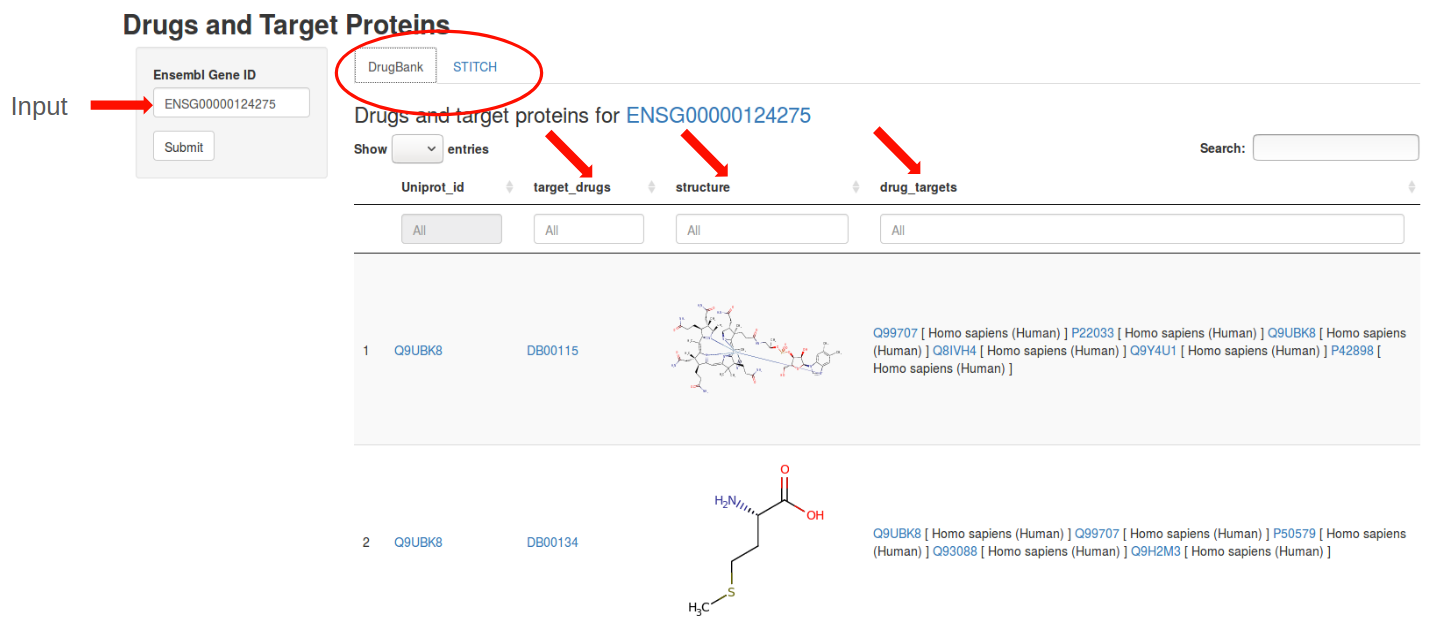
\includegraphics[width=10.5cm]{demo/images/shiny.png}
    \end{figure}
\vspace{-0.5cm}
\textcolor{blue}{Application:} \\
query for drug-target annotations in DrugBank and STITCH databases online \\
\end{frame}
%%%%%%%%%%%%%%%%%%%%%%%%%%%%%%%%% SLIDE %%%%%%%%%%%%%%%%%%%%%%%%%%%%%%%%%
\section{Acknowledgement}
%%%%%%%%%%%%%%%%%%%%%%%%%%%%%%%%% SLIDE %%%%%%%%%%%%%%%%%%%%%%%%%%%%%%%%%
\begin{frame}{Acknowledgement}
\vspace{-1.6cm}
\textcolor{blue}{Instructor:} \\
Dr. Thomas Girke \\
\vspace{0.6cm}
\textcolor{blue}{Lab members:} \\
Daniela Cassol, Jianhai Zhang \\
\vspace{0.6cm}
\textcolor{blue}{Funding Source:} \\ 
NIH, NIA
\end{frame}
%%%%%%%%%%%%%%%%%%%%%%%%%%%%%%%%% SLIDE %%%%%%%%%%%%%%%%%%%%%%%%%%%%%%%%%
\begin{frame}[standout]
  Questions?
\end{frame}
%%%%%%%%%%%%%%%%%%%%%%%%%%%%%%%%% SLIDE %%%%%%%%%%%%%%%%%%%%%%%%%%%%%%%%%
\appendix
%%%%%%%%%%%%%%%%%%%%%%%%%%%%%%%%% SLIDE %%%%%%%%%%%%%%%%%%%%%%%%%%%%%%%%%
\begin{frame}[fragile]{Progress on GESS}
%  \begin{table}
%  %\rowcolors{1}{}{blue}
%    \begin{tabular}{ccccccc}
%      \hline
%      \footnotesize
%      group & year & reference database & gess methods & organism & contribution & limitation \\
%      \hline
%      \cite{hughes2000-iz} & 2000 & 300 diverse mutations and chemical treatments & hierarchical clustering on error-weighted correlation coefficient & \textcolor{blue}{yeast} & demonstrate utility of gess in yeast & \\
%      \cite{ganter2005-or} & 2005 & 600 drug treatments & hierarchical clustering on expression correlation & \textcolor{blue}{rat} & demonstrate utility of gess in rat tissues & could not scale up: compound type; high cost\\
%      %\cite{lamb2006-du} & 2006  2017 & \textcolor{blue}{\textbf{cmap-affy}} \textcolor{blue}{\textbf{cmap-l1000}} & \textcolor{blue}{\textbf{cmap}}  \textcolor{blue}{\textbf{cmap-lincs}} & human cancer cell & demonstrate utility of gess in mammalian cell culture; introduce \textcolor{blue}{cmap} & \\
%      \hline
%    \end{tabular}
%  \end{table}
\vspace{-1cm}
\begin{figure}
    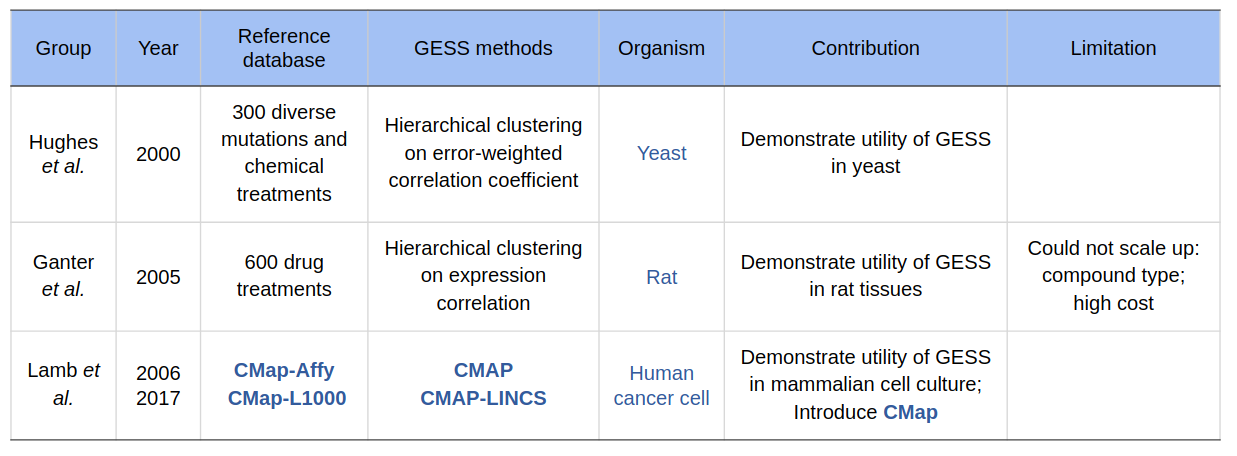
\includegraphics[width=11.2cm]{demo/images/progress_gess.png}
\end{figure}
\end{frame}
%%%%%%%%%%%%%%%%%%%%%%%%%%%%%%%%% SLIDE %%%%%%%%%%%%%%%%%%%%%%%%%%%%%%%%%
\begin{frame}[fragile]{Backup slides}
    \begin{figure}
        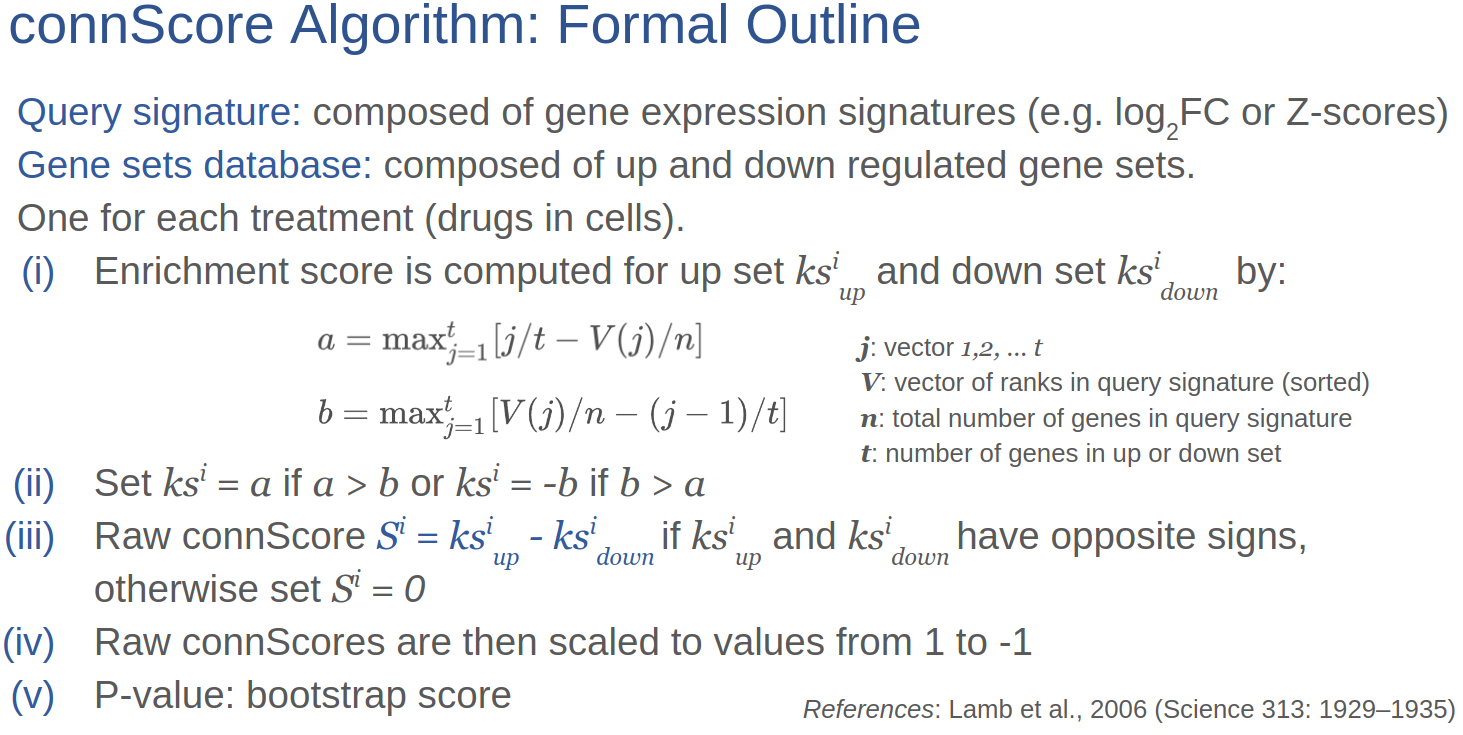
\includegraphics[width=12cm]{demo/images/connScore_algo.png}
    \end{figure}
\end{frame}
%%%%%%%%%%%%%%%%%%%%%%%%%%%%%%%%% SLIDE %%%%%%%%%%%%%%%%%%%%%%%%%%%%%%%%%
\begin{frame}[fragile]{Backup slides}
    \begin{figure}
        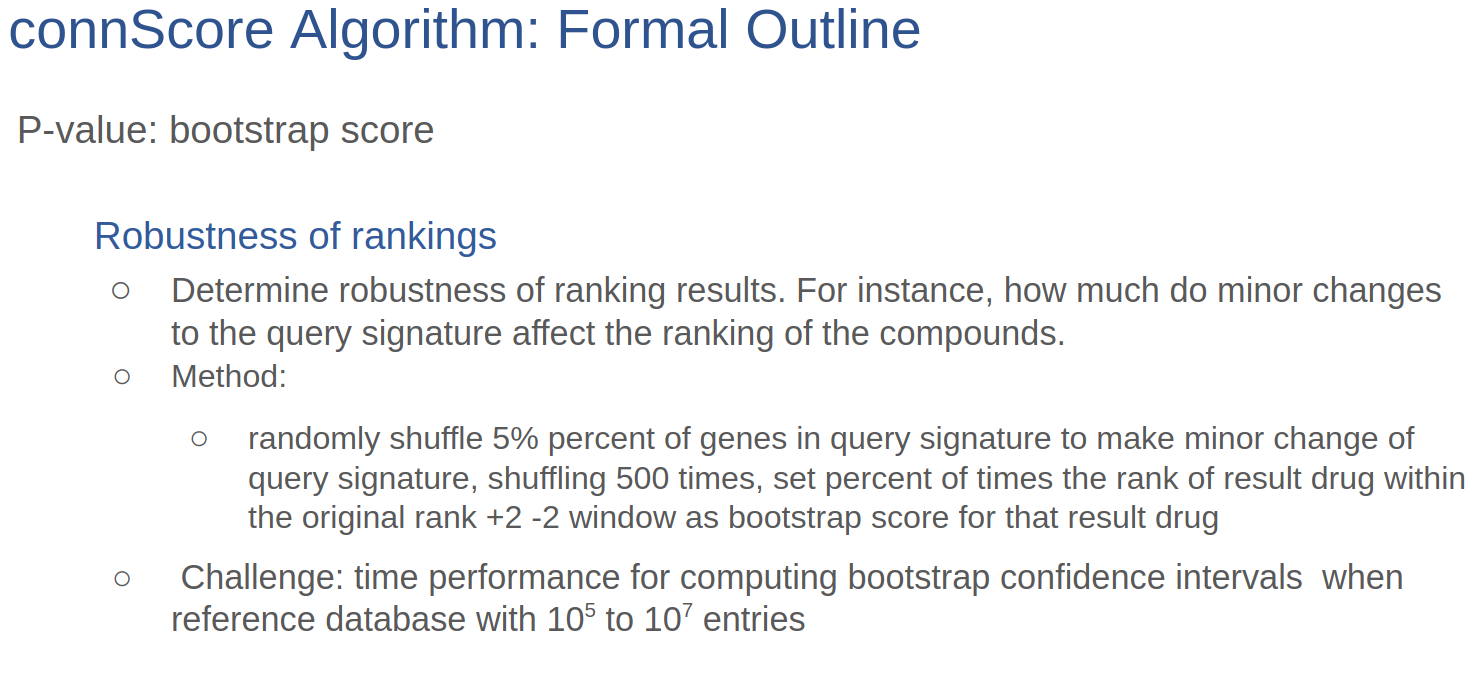
\includegraphics[width=11cm]{demo/images/connScore_algo2.png}
    \end{figure}
\end{frame}
%%%%%%%%%%%%%%%%%%%%%%%%%%%%%%%%% SLIDE %%%%%%%%%%%%%%%%%%%%%%%%%%%%%%%%%
\begin{frame}[fragile]{Backup slides}
    \begin{figure}
        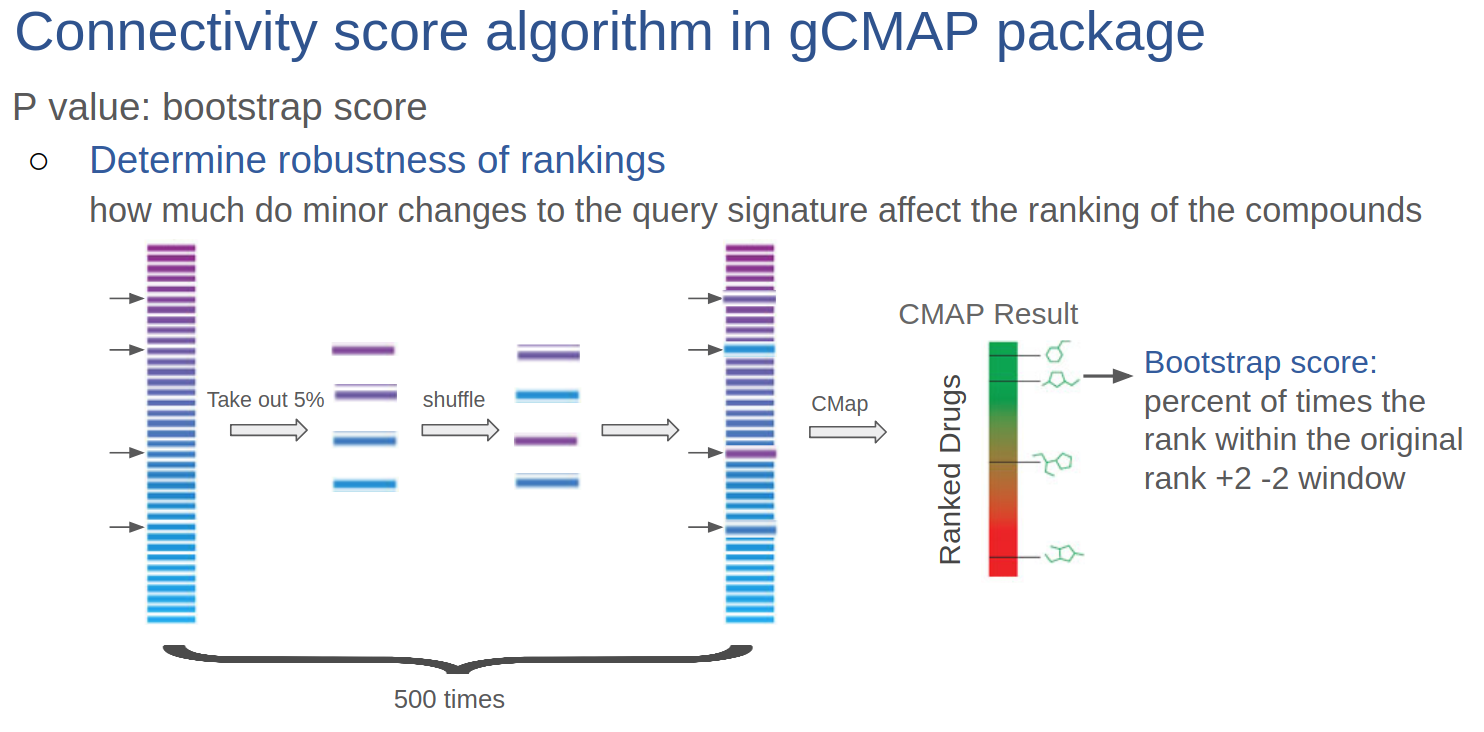
\includegraphics[width=12cm]{demo/images/connScore_boot_score.png}
    \end{figure}
\end{frame}
%%%%%%%%%%%%%%%%%%%%%%%%%%%%%%%%% SLIDE %%%%%%%%%%%%%%%%%%%%%%%%%%%%%%%%%
\begin{frame}[fragile]{Backup slides}
    \begin{figure}
        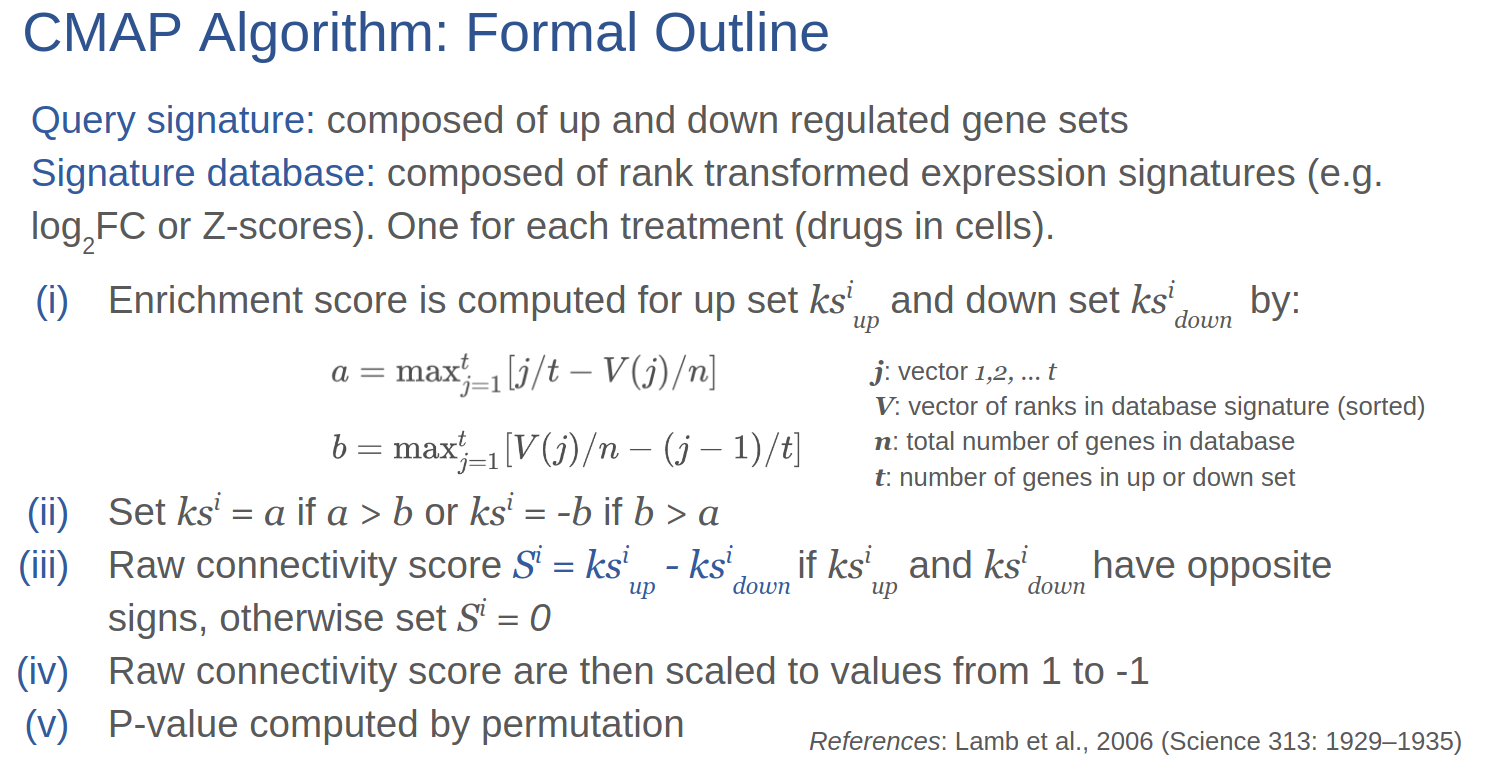
\includegraphics[width=12cm]{demo/images/cmap_algo.png}
    \end{figure}
\end{frame}
%%%%%%%%%%%%%%%%%%%%%%%%%%%%%%%%% SLIDE %%%%%%%%%%%%%%%%%%%%%%%%%%%%%%%%%
\begin{frame}[fragile]{Backup slides}
    \begin{figure}
        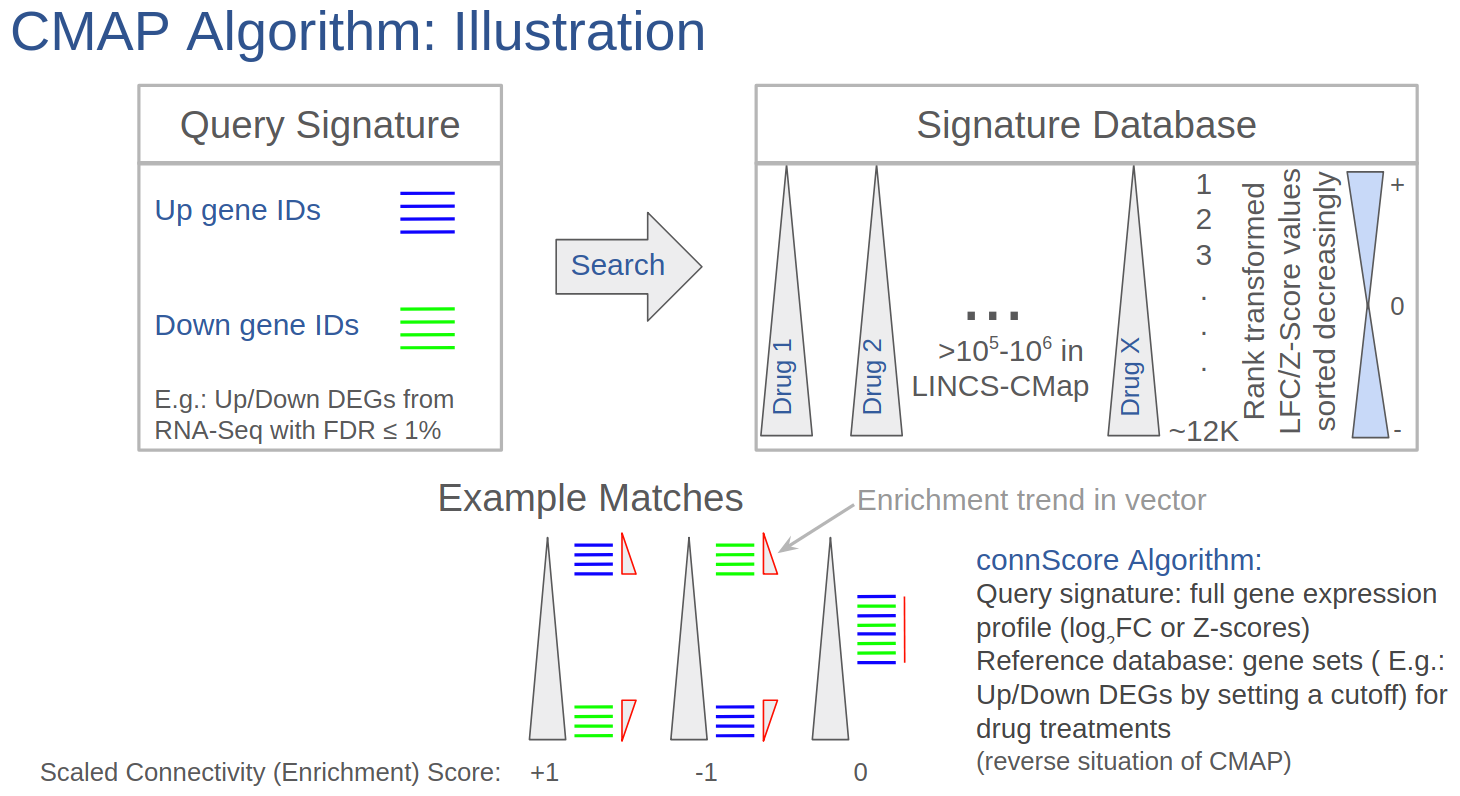
\includegraphics[width=12cm]{demo/images/cmap_algo_illu.png}
    \end{figure}
\end{frame}
%%%%%%%%%%%%%%%%%%%%%%%%%%%%%%%%% SLIDE %%%%%%%%%%%%%%%%%%%%%%%%%%%%%%%%%
\begin{frame}[fragile]{Backup slides}
    \begin{figure}
        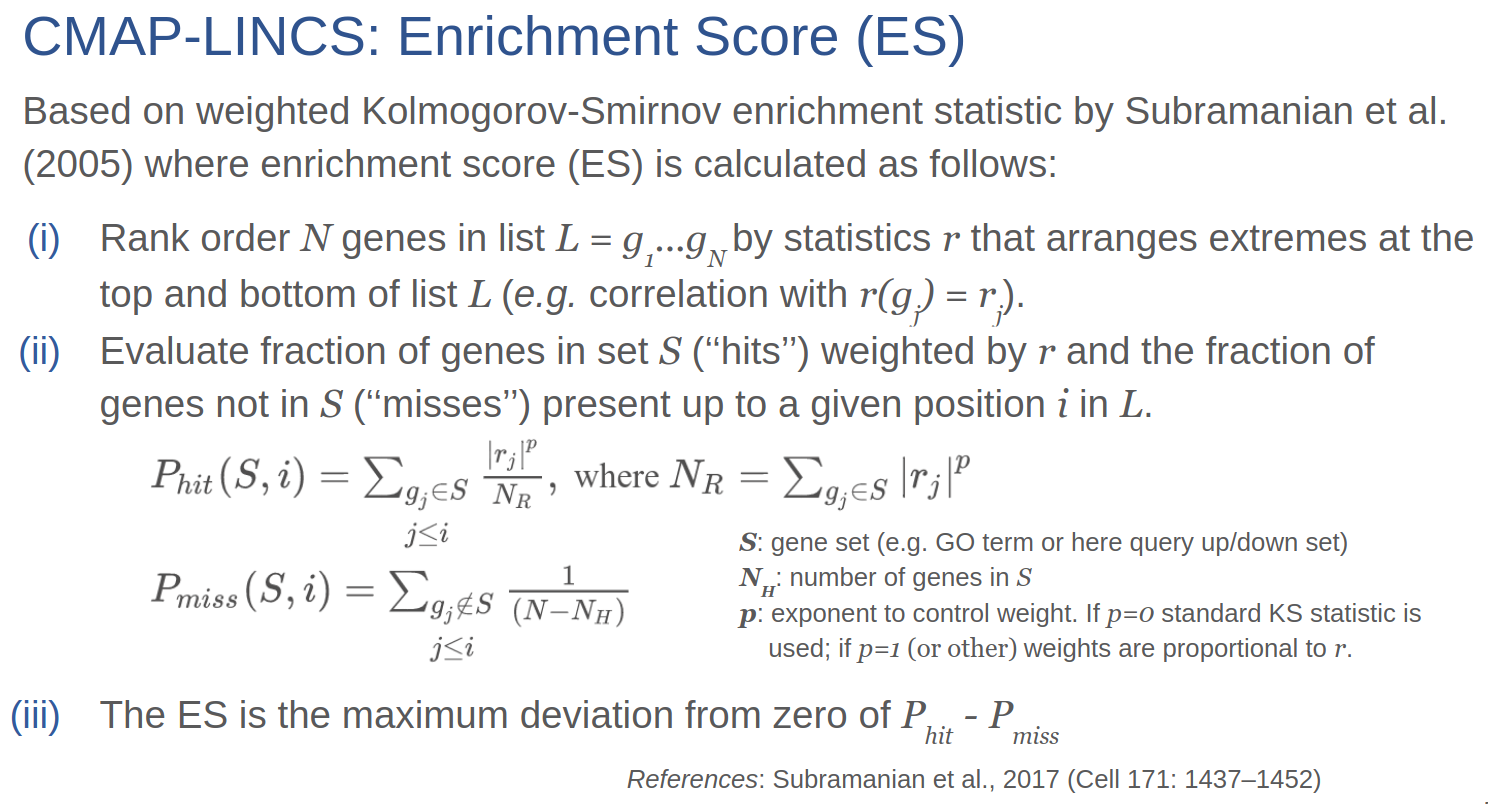
\includegraphics[width=11cm]{demo/images/cmap_lincs_algo.png}
    \end{figure}
\end{frame}
%%%%%%%%%%%%%%%%%%%%%%%%%%%%%%%%% SLIDE %%%%%%%%%%%%%%%%%%%%%%%%%%%%%%%%%
\begin{frame}[fragile]{Backup slides}
    \begin{figure}
        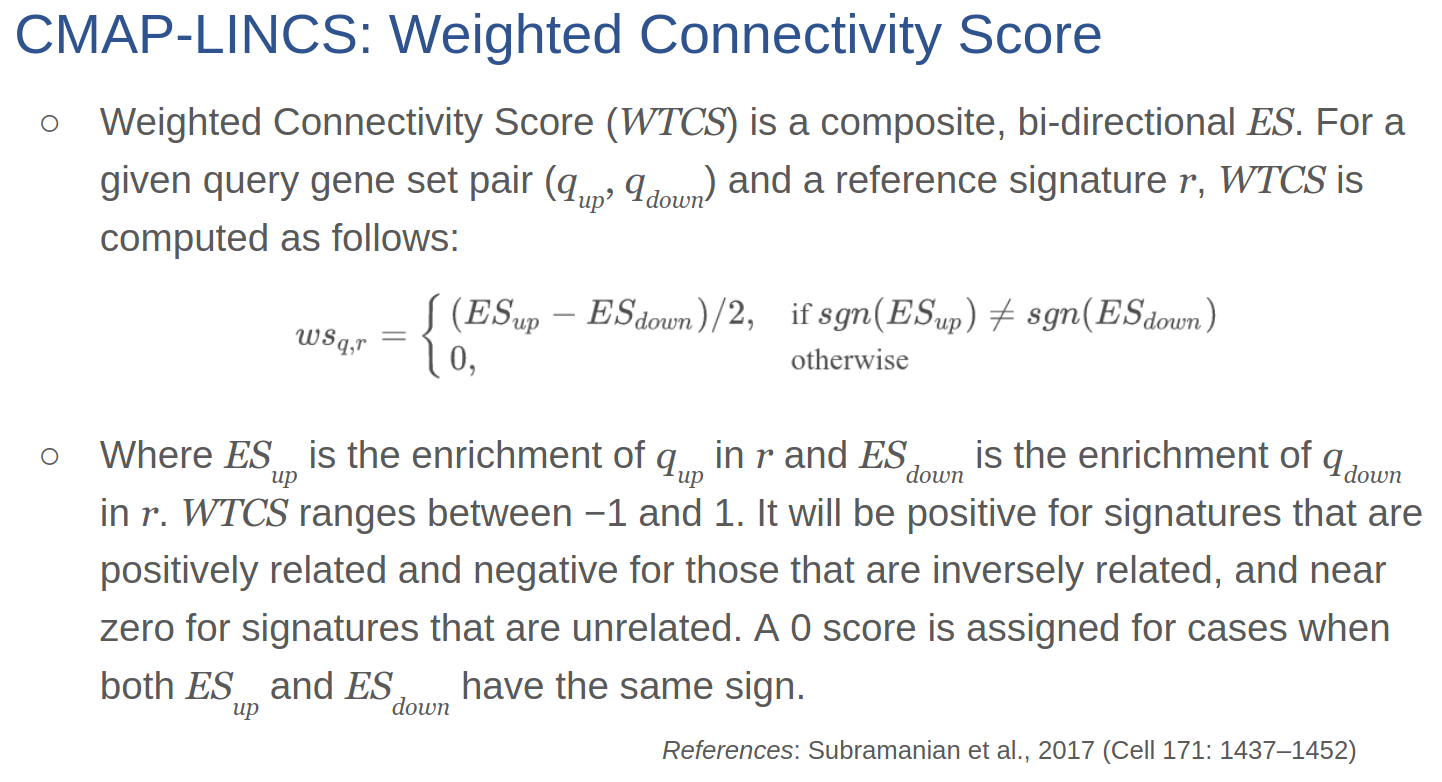
\includegraphics[width=12cm]{demo/images/cmap_lincs_wtcs.png}
    \end{figure}
\end{frame}
%%%%%%%%%%%%%%%%%%%%%%%%%%%%%%%%% SLIDE %%%%%%%%%%%%%%%%%%%%%%%%%%%%%%%%%
\begin{frame}[fragile]{Backup slides}
    \begin{figure}
        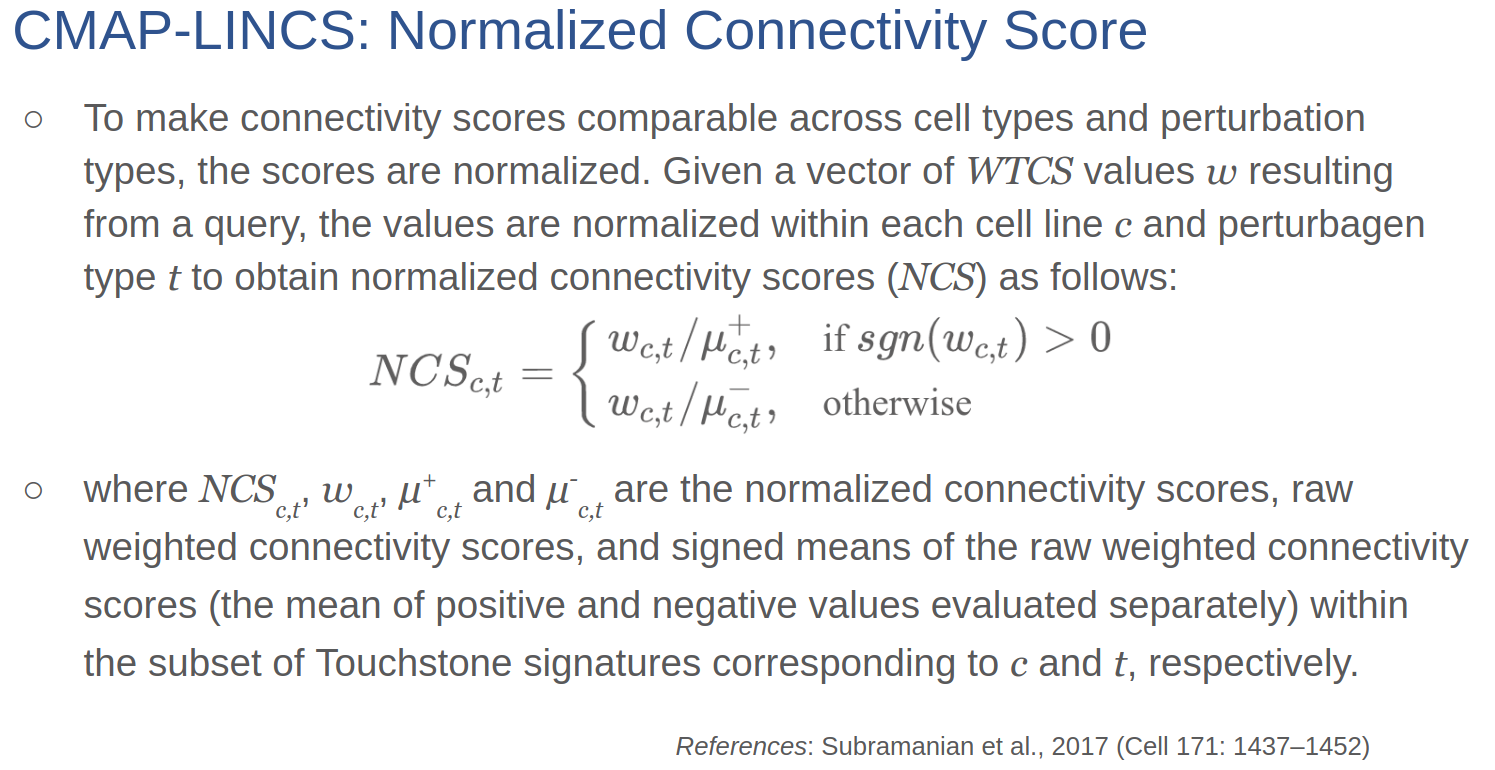
\includegraphics[width=12cm]{demo/images/cmap_lincs_ncs.png}
    \end{figure}
\end{frame}
%%%%%%%%%%%%%%%%%%%%%%%%%%%%%%%%% SLIDE %%%%%%%%%%%%%%%%%%%%%%%%%%%%%%%%%
\begin{frame}[fragile]{Backup slides}
    \begin{figure}
        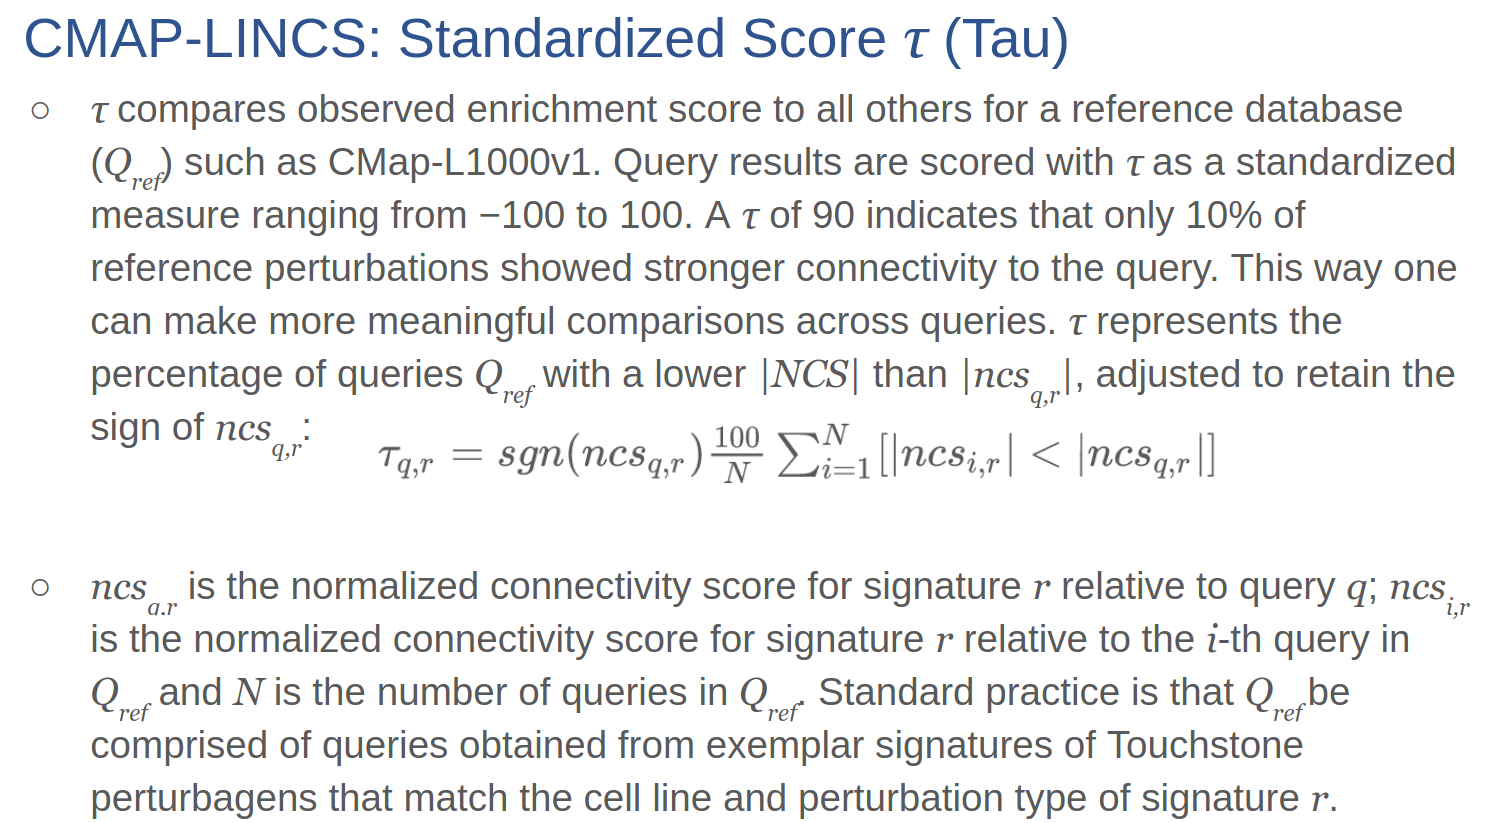
\includegraphics[width=12cm]{demo/images/cmap_lincs_tau.png}
    \end{figure}
\end{frame}
%%%%%%%%%%%%%%%%%%%%%%%%%%%%%%%%% SLIDE %%%%%%%%%%%%%%%%%%%%%%%%%%%%%%%%%
\begin{frame}[fragile]{Backup slides}
    \begin{figure}
        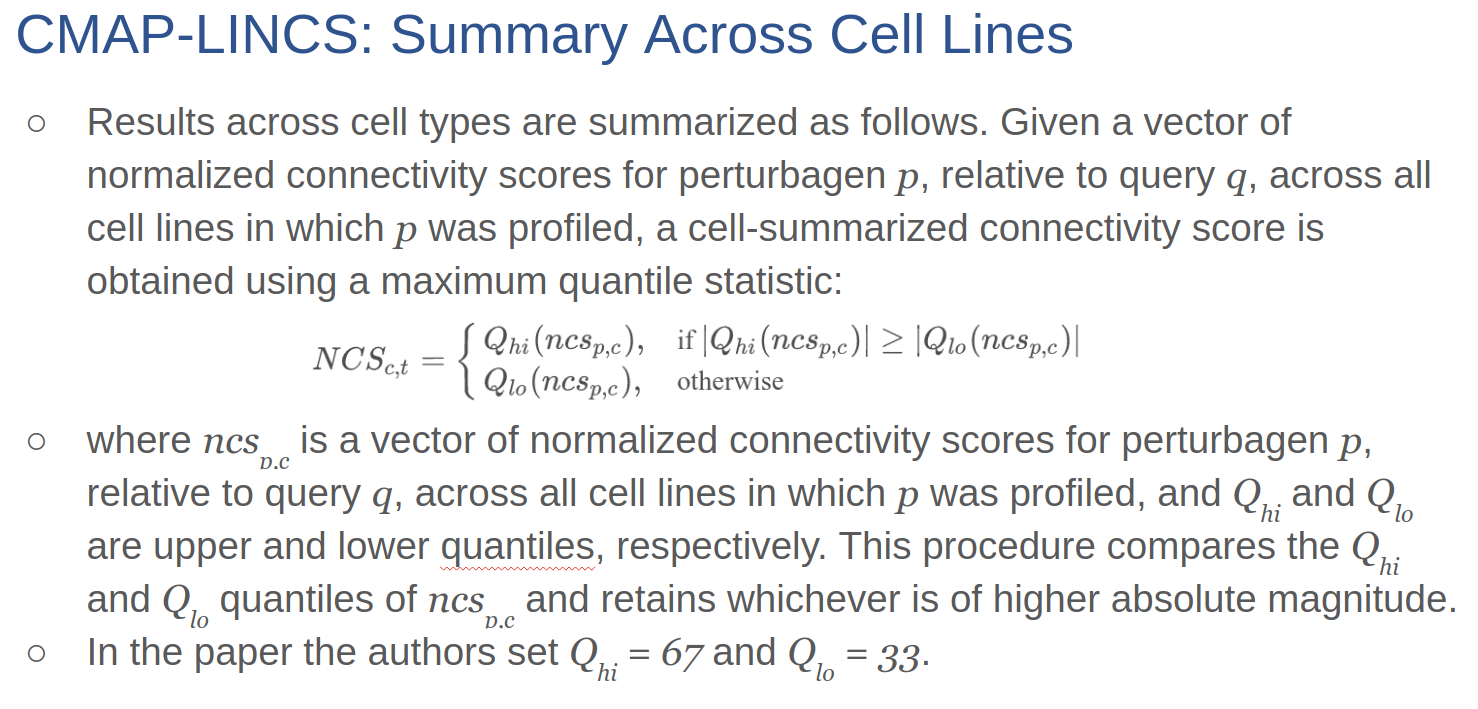
\includegraphics[width=12cm]{demo/images/cmap_lincs_ncsct.png}
    \end{figure}
\end{frame}
%%%%%%%%%%%%%%%%%%%%%%%%%%%%%%%%% SLIDE %%%%%%%%%%%%%%%%%%%%%%%%%%%%%%%%%
\begin{frame}[fragile]{Backup slides}
    \begin{figure}
        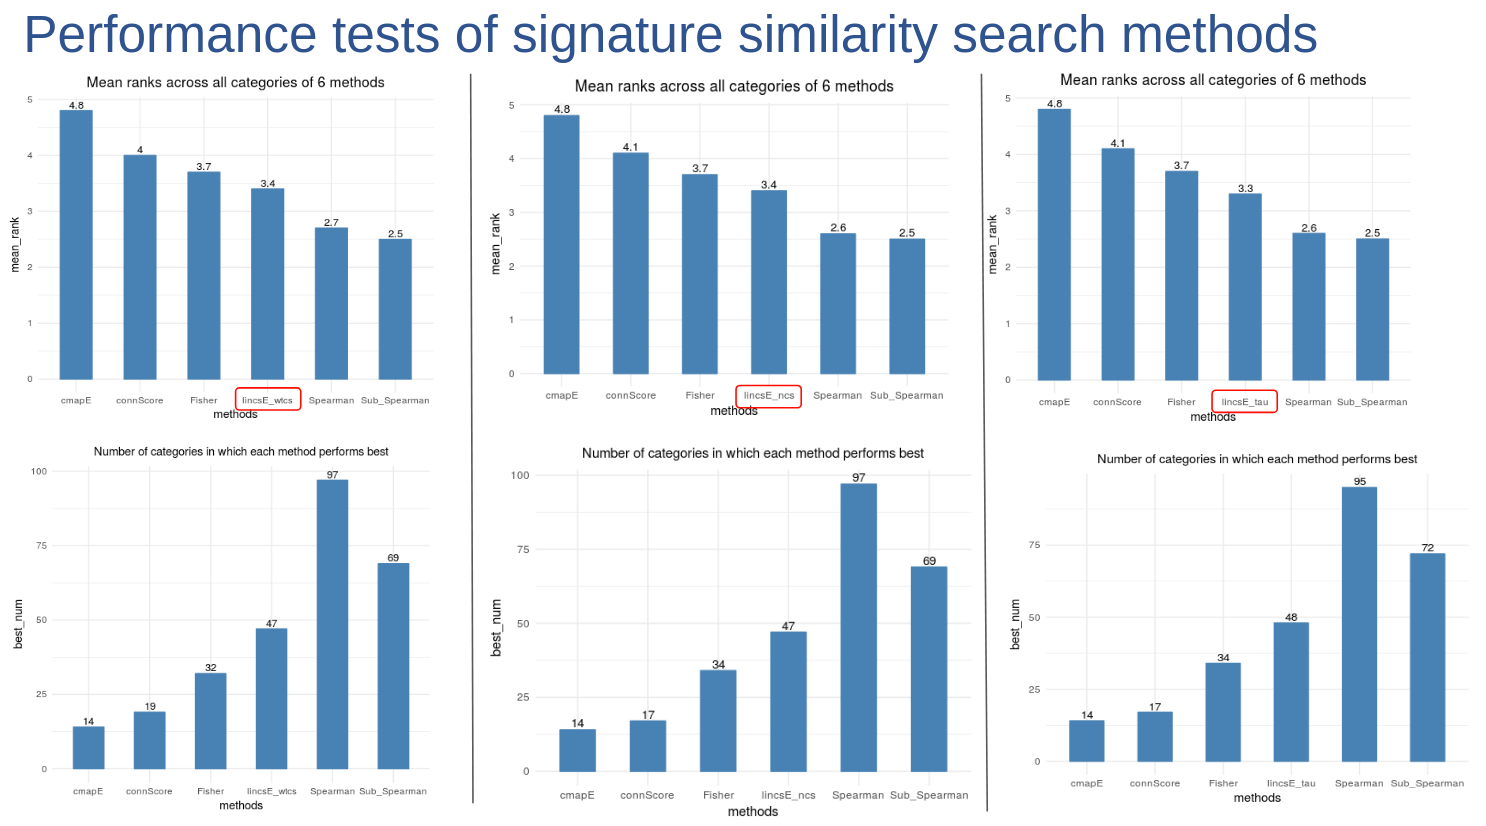
\includegraphics[width=12cm]{demo/images/gess_test_3_lincs_score.png}
    \end{figure}
\end{frame}
%%%%%%%%%%%%%%%%%%%%%%%%%%%%%%%%% SLIDE %%%%%%%%%%%%%%%%%%%%%%%%%%%%%%%%%
\begin{frame}[fragile]{Backup slides}
    \begin{figure}
        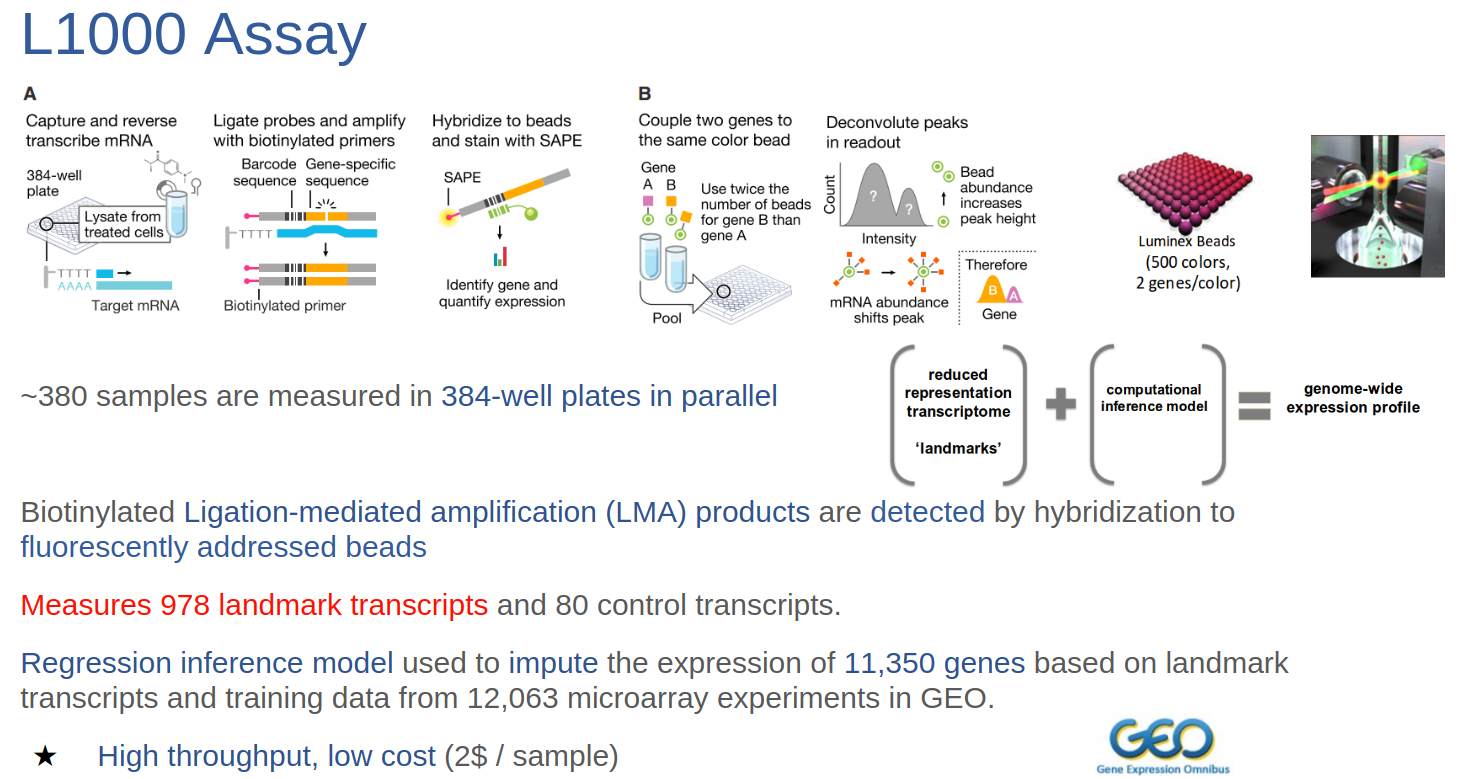
\includegraphics[width=12cm]{demo/images/l1000_assay.png}
    \end{figure}
\end{frame}
%%%%%%%%%%%%%%%%%%%%%%%%%%%%%%%%% SLIDE %%%%%%%%%%%%%%%%%%%%%%%%%%%%%%%%%
\begin{frame}[fragile]{Backup slides}
    \begin{figure}
        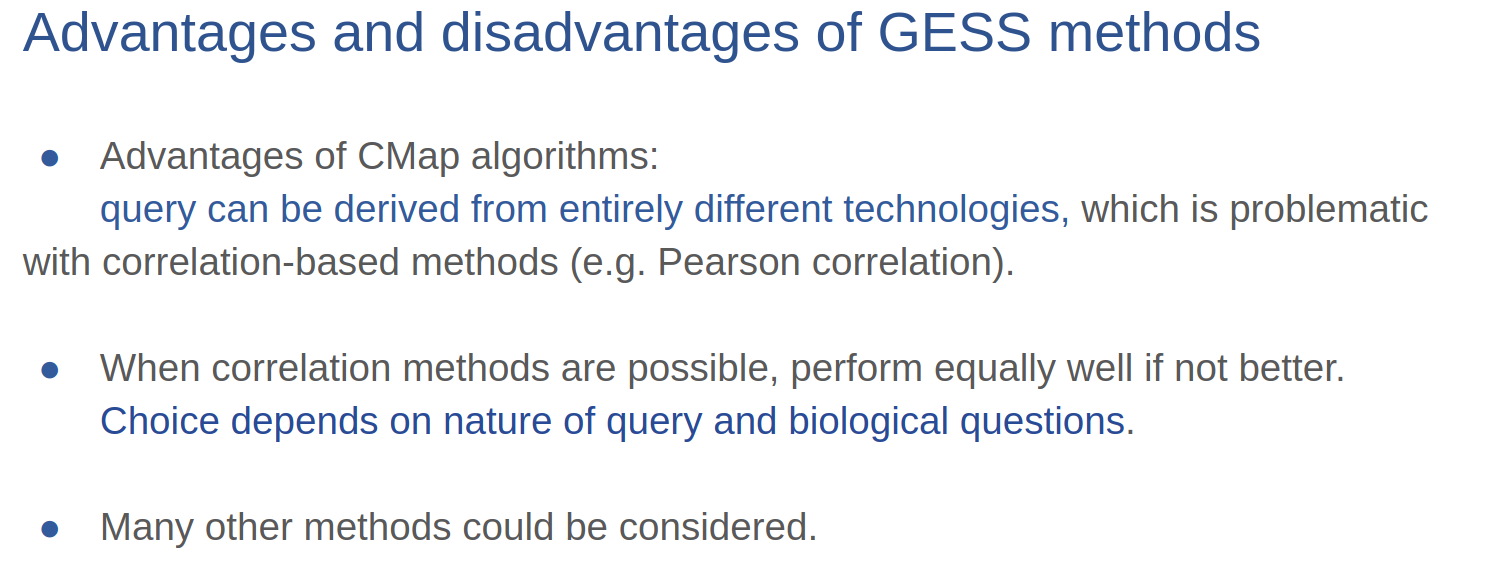
\includegraphics[width=12cm]{demo/images/ad_disad_gess.png}
    \end{figure}
\end{frame}
%%%%%%%%%%%%%%%%%%%%%%%%%%%%%%%%% SLIDE %%%%%%%%%%%%%%%%%%%%%%%%%%%%%%%%%
\begin{frame}[fragile]{Backup slides}
    \begin{figure}
        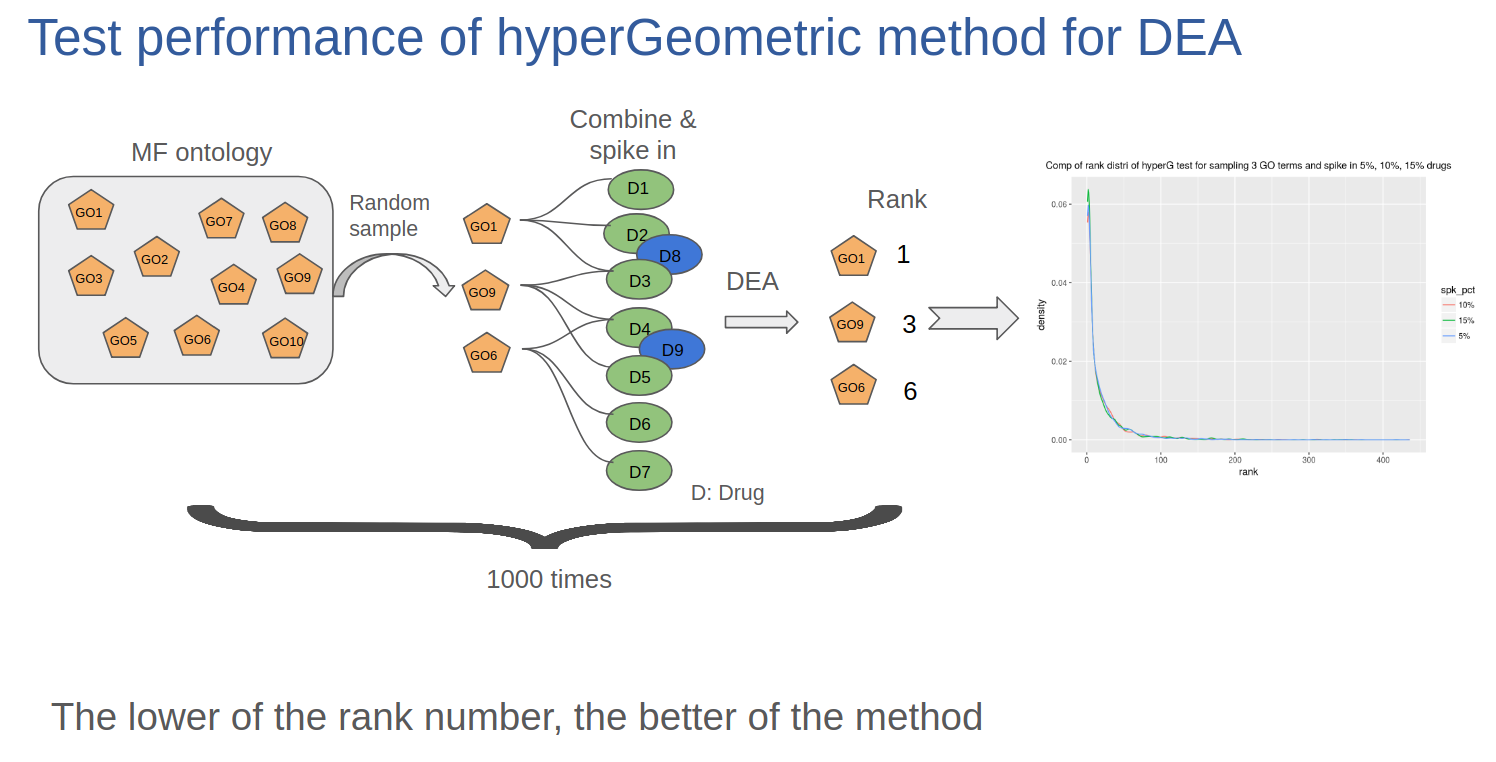
\includegraphics[width=12cm]{demo/images/test_perform_hyperG.png}
    \end{figure}
\end{frame}
%%%%%%%%%%%%%%%%%%%%%%%%%%%%%%%%% SLIDE %%%%%%%%%%%%%%%%%%%%%%%%%%%%%%%%%
\begin{frame}[fragile]{Backup slides}
    \begin{figure}
        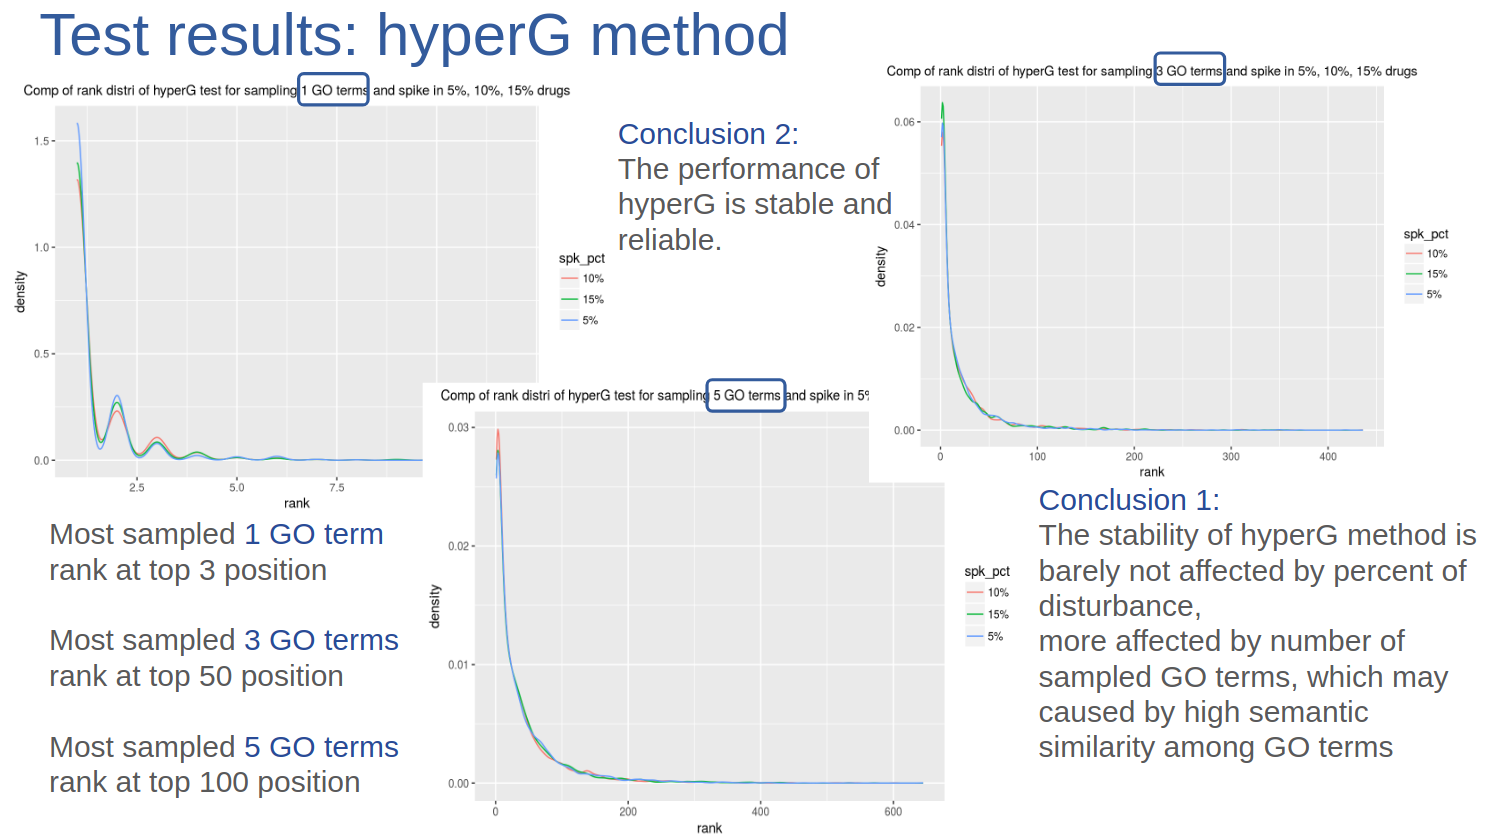
\includegraphics[width=12cm]{demo/images/test_perform_hyperG_res.png}
    \end{figure}
\end{frame}
%%%%%%%%%%%%%%%%%%%%%%%%%%%%%%%%% SLIDE %%%%%%%%%%%%%%%%%%%%%%%%%%%%%%%%%
\begin{frame}[fragile]{Backup slides}
    \begin{figure}
        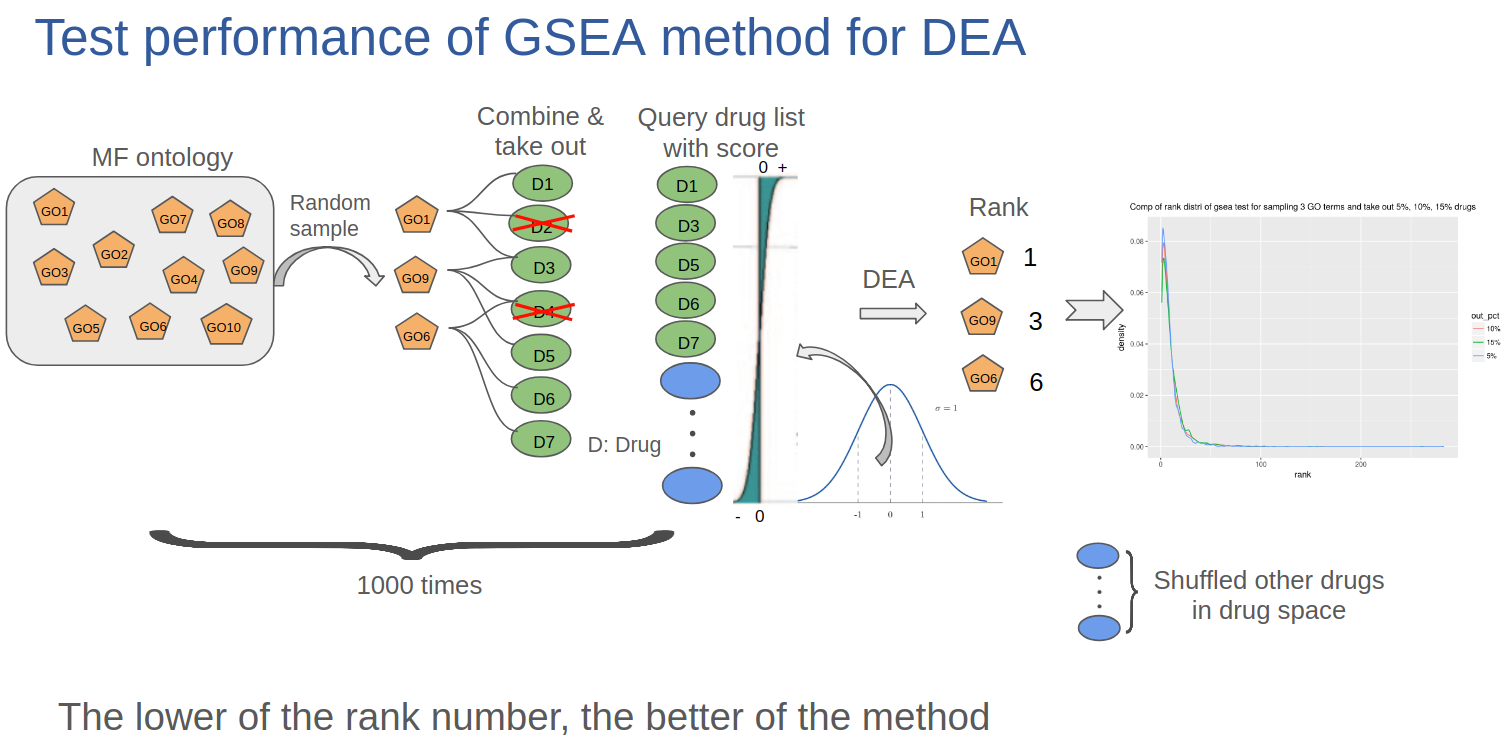
\includegraphics[width=12cm]{demo/images/test_perform_gsea.png}
    \end{figure}
\end{frame}
%%%%%%%%%%%%%%%%%%%%%%%%%%%%%%%%% SLIDE %%%%%%%%%%%%%%%%%%%%%%%%%%%%%%%%%
\begin{frame}[fragile]{Backup slides}
    \begin{figure}
        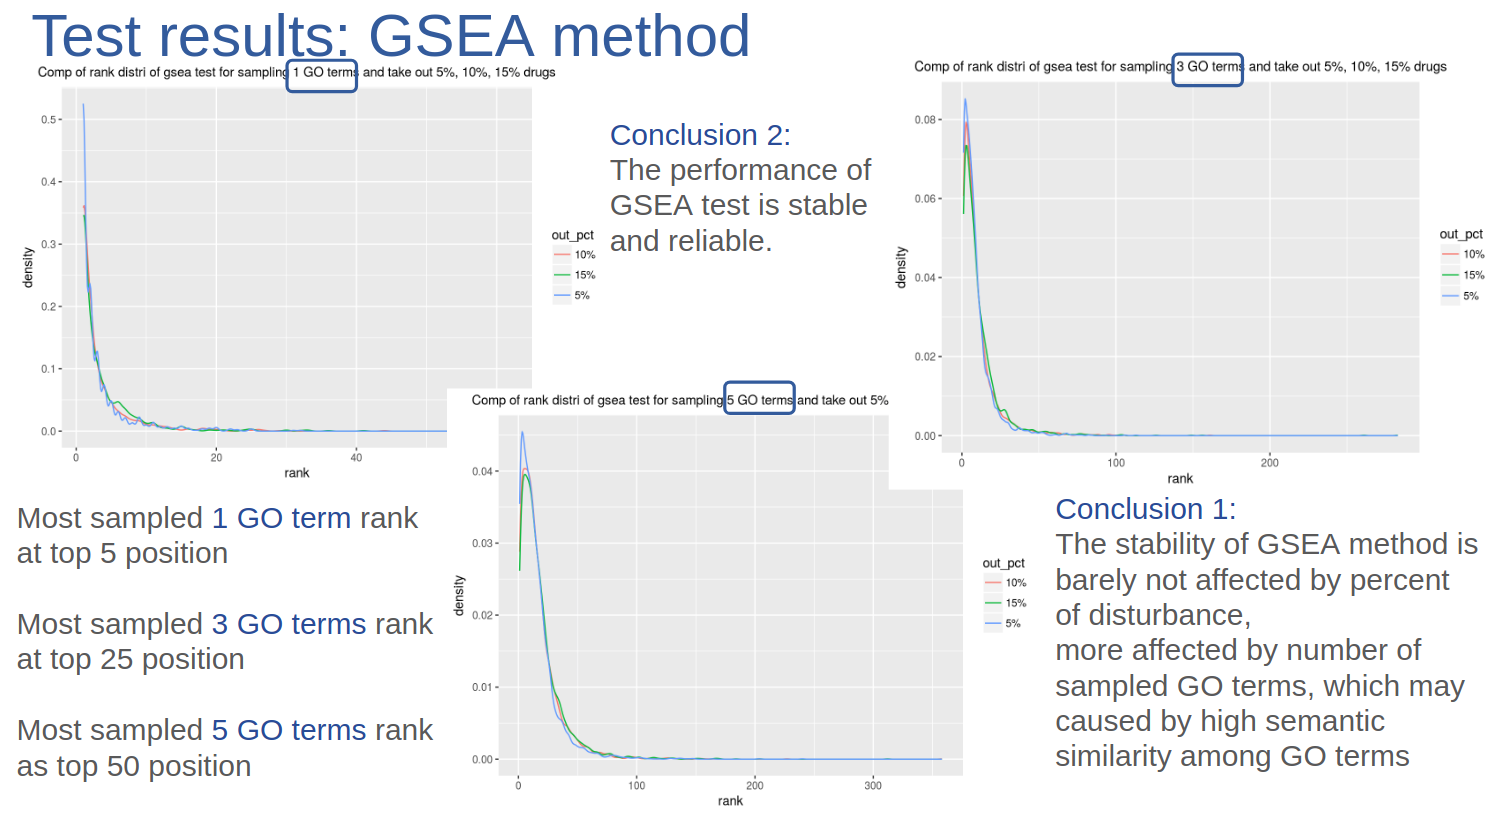
\includegraphics[width=12cm]{demo/images/test_perform_gsea_res.png}
    \end{figure}
\end{frame}
%%%%%%%%%%%%%%%%%%%%%%%%%%%%%%%%% SLIDE %%%%%%%%%%%%%%%%%%%%%%%%%%%%%%%%%
\begin{frame}[fragile]{Backup slides}
    \begin{figure}
        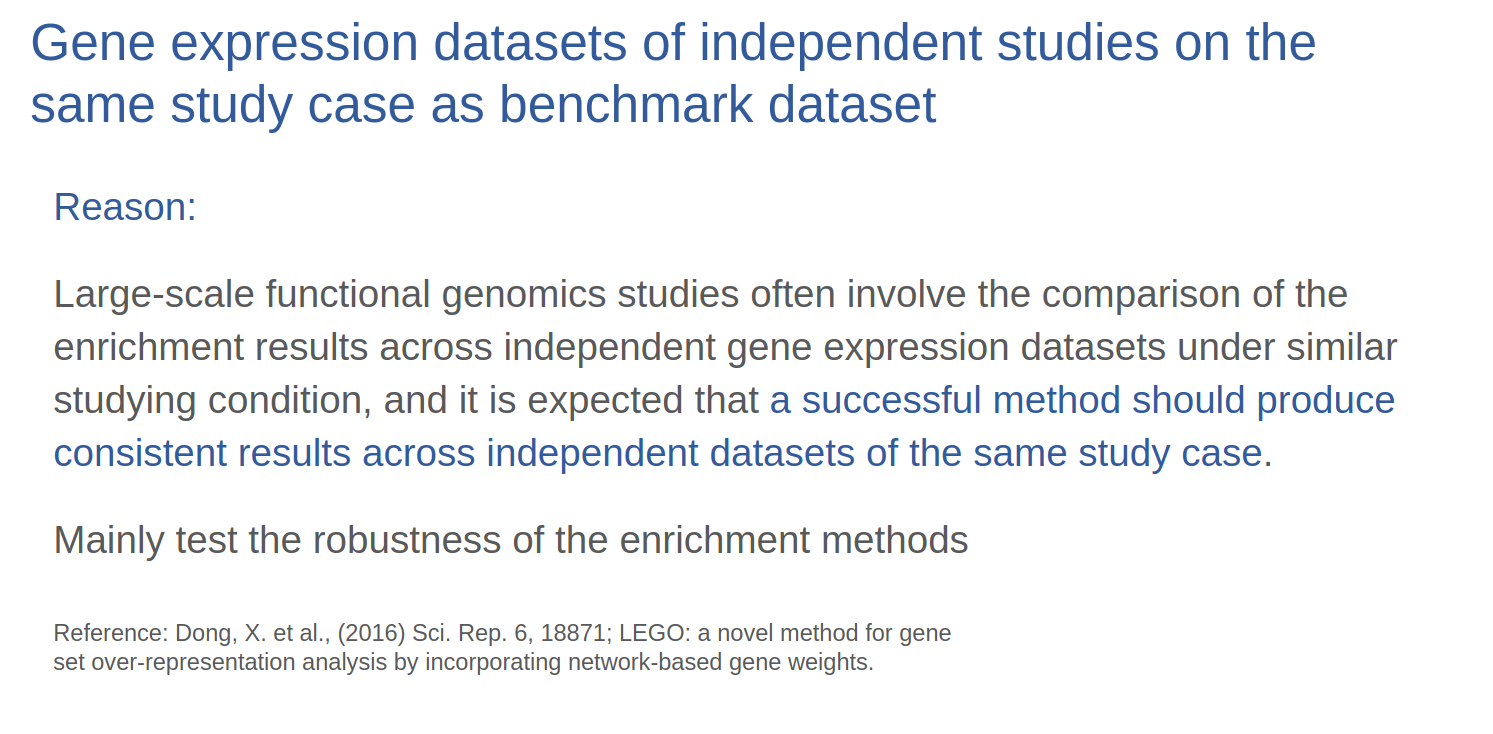
\includegraphics[width=12cm]{demo/images/ind_case1.png}
    \end{figure}
\end{frame}
%%%%%%%%%%%%%%%%%%%%%%%%%%%%%%%%% SLIDE %%%%%%%%%%%%%%%%%%%%%%%%%%%%%%%%%
\begin{frame}[fragile]{Backup slides}
    \begin{figure}
        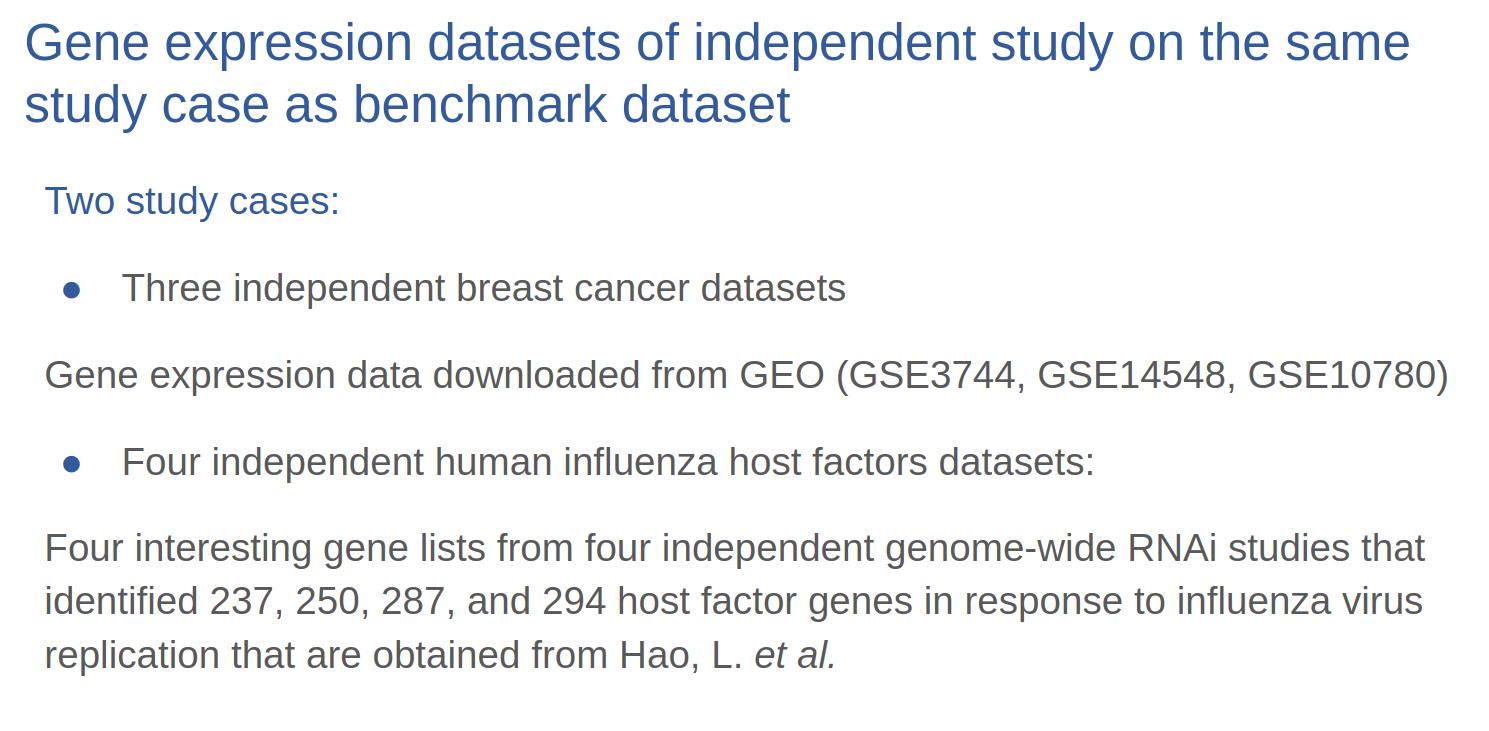
\includegraphics[width=12cm]{demo/images/ind_case2.png}
    \end{figure}
\end{frame}
%%%%%%%%%%%%%%%%%%%%%%%%%%%%%%%%% SLIDE %%%%%%%%%%%%%%%%%%%%%%%%%%%%%%%%%
\begin{frame}[fragile]{Backup slides}
    \begin{figure}
        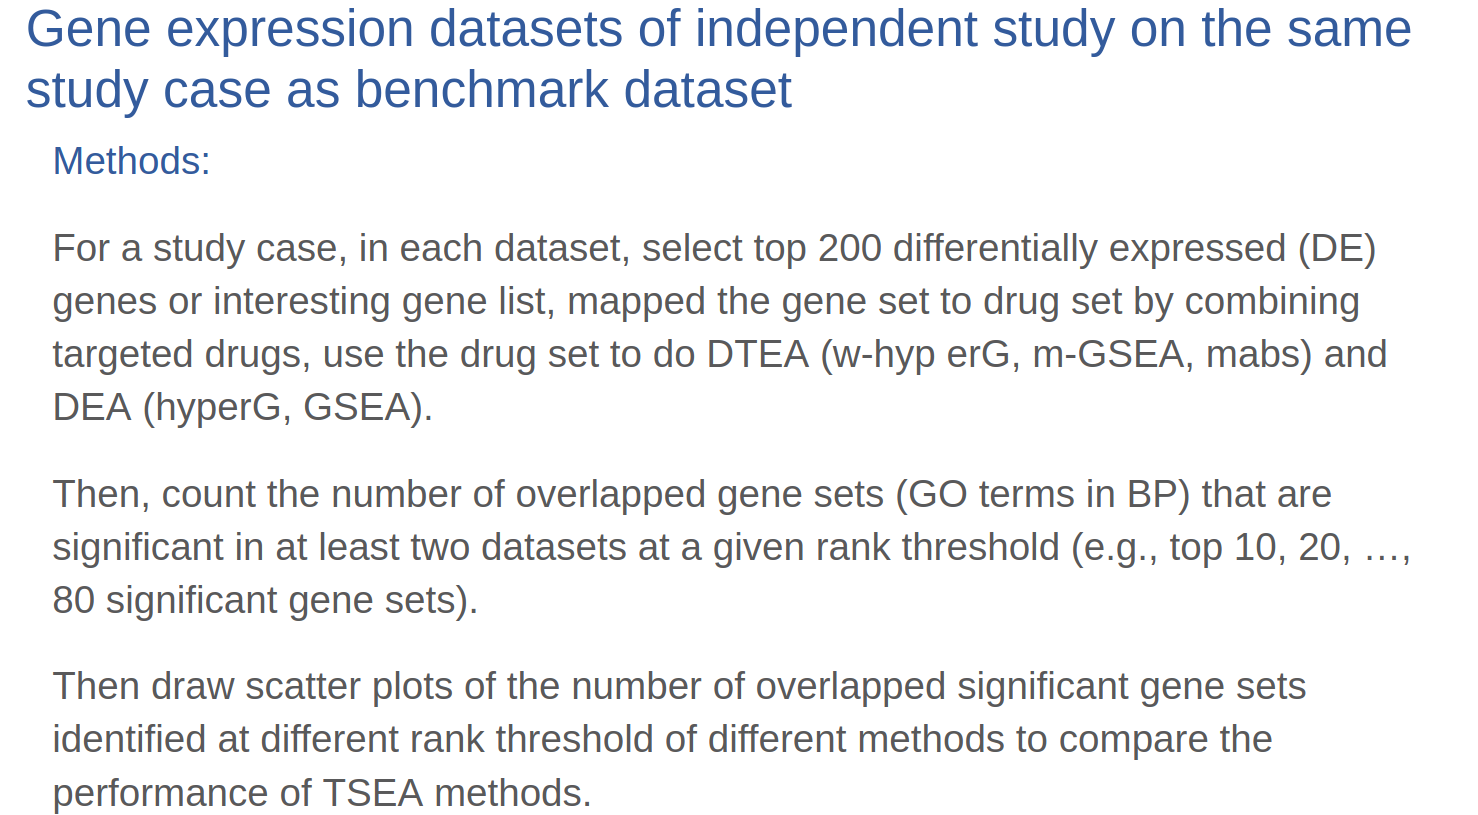
\includegraphics[width=12cm]{demo/images/ind_case3.png}
    \end{figure}
\end{frame}
%%%%%%%%%%%%%%%%%%%%%%%%%%%%%%%%% SLIDE %%%%%%%%%%%%%%%%%%%%%%%%%%%%%%%%%
\begin{frame}[fragile]{Backup slides}
    \begin{figure}
        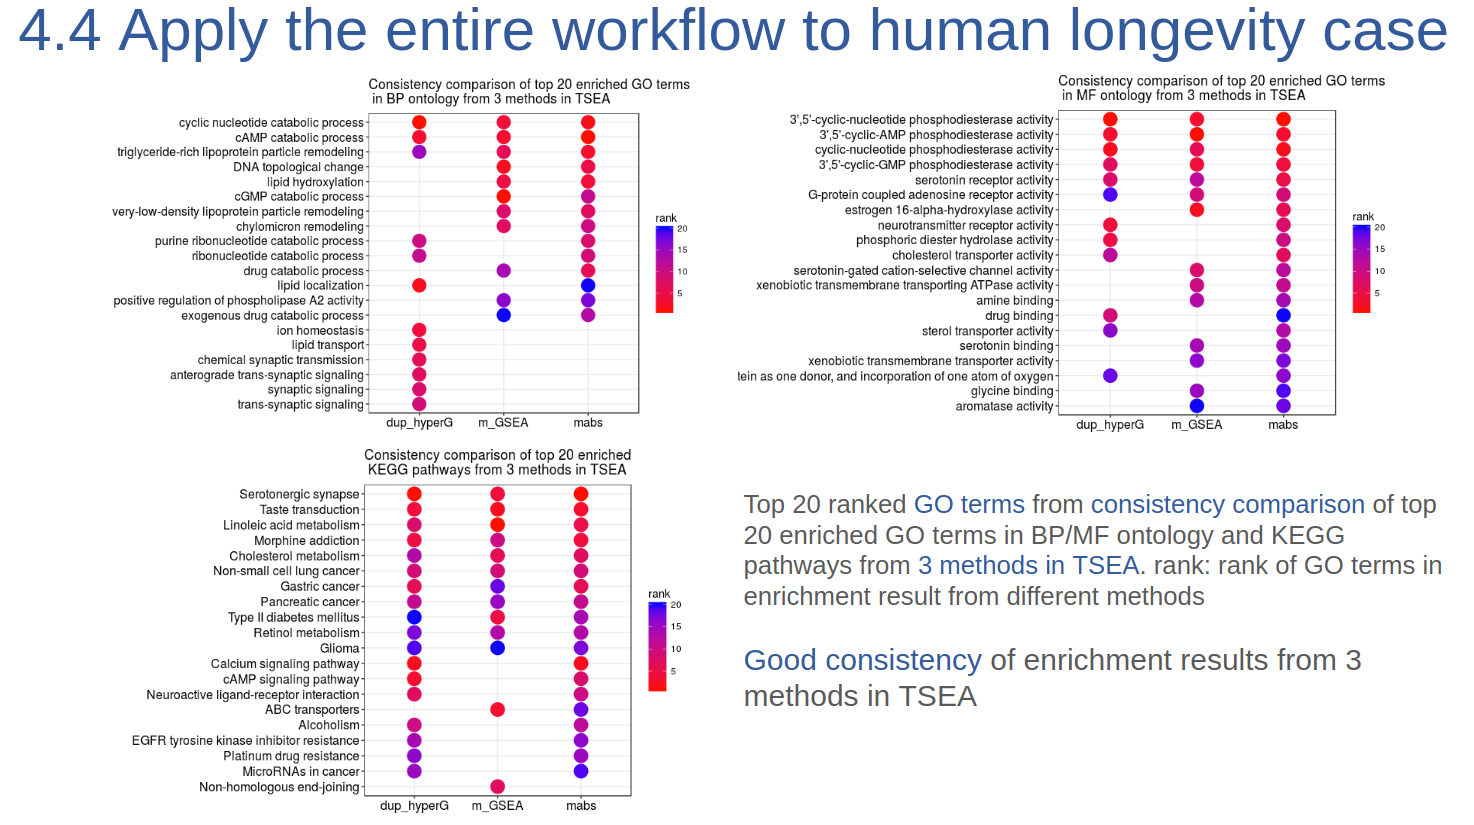
\includegraphics[width=12cm]{demo/images/cmp_tsea_methods.png}
    \end{figure}
\end{frame}
%%%%%%%%%%%%%%%%%%%%%%%%%%%%%%%%% SLIDE %%%%%%%%%%%%%%%%%%%%%%%%%%%%%%%%%
\begin{frame}[fragile]{Backup slides}
    \begin{figure}
        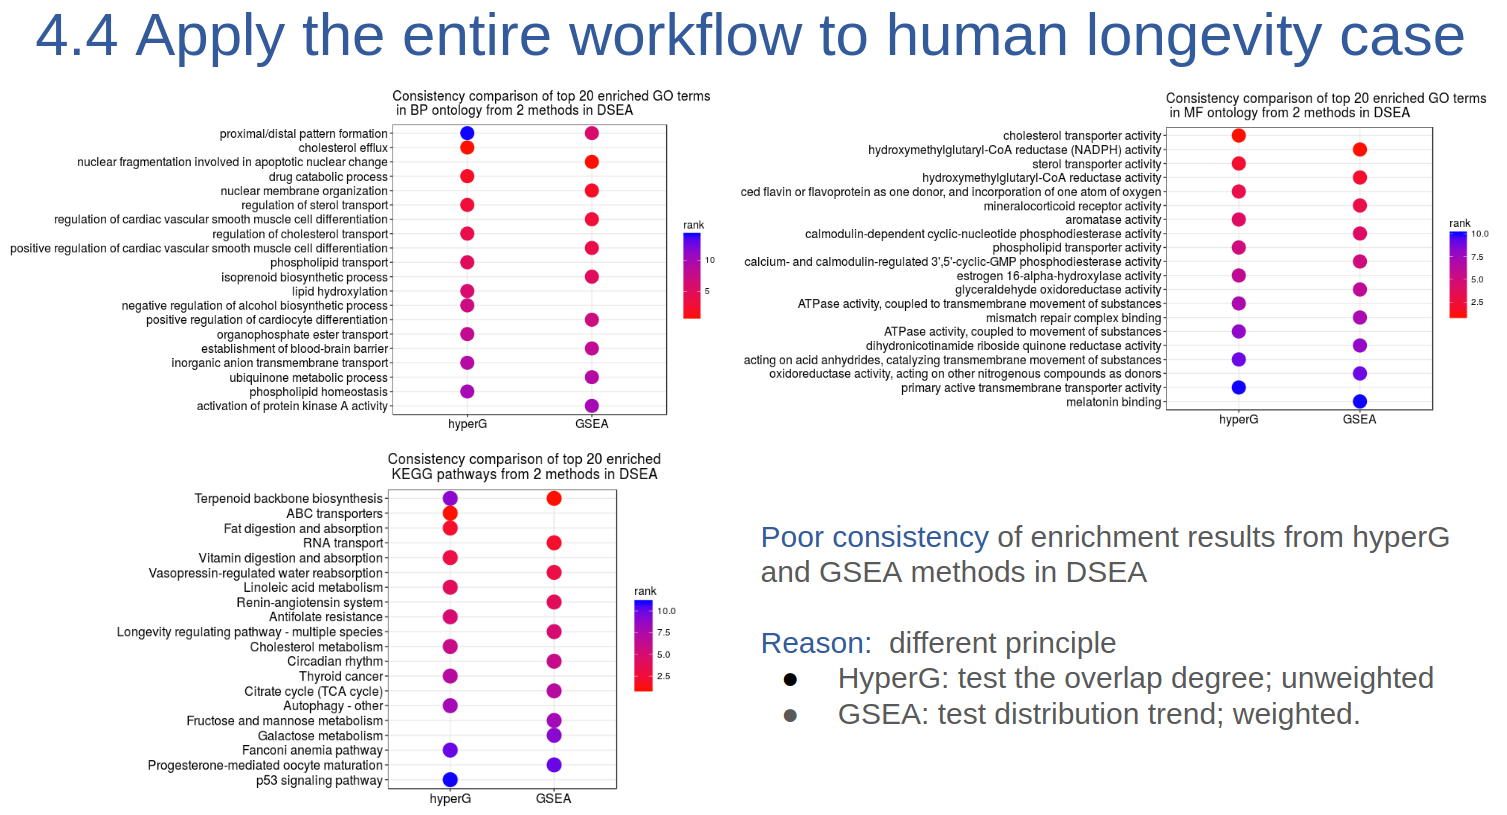
\includegraphics[width=12cm]{demo/images/cmp_dsea_methods.png}
    \end{figure}
\end{frame}
%%%%%%%%%%%%%%%%%%%%%%%%%%%%%%%%% SLIDE %%%%%%%%%%%%%%%%%%%%%%%%%%%%%%%%%
\begin{frame}{Backup slides}
    \begin{figure}
        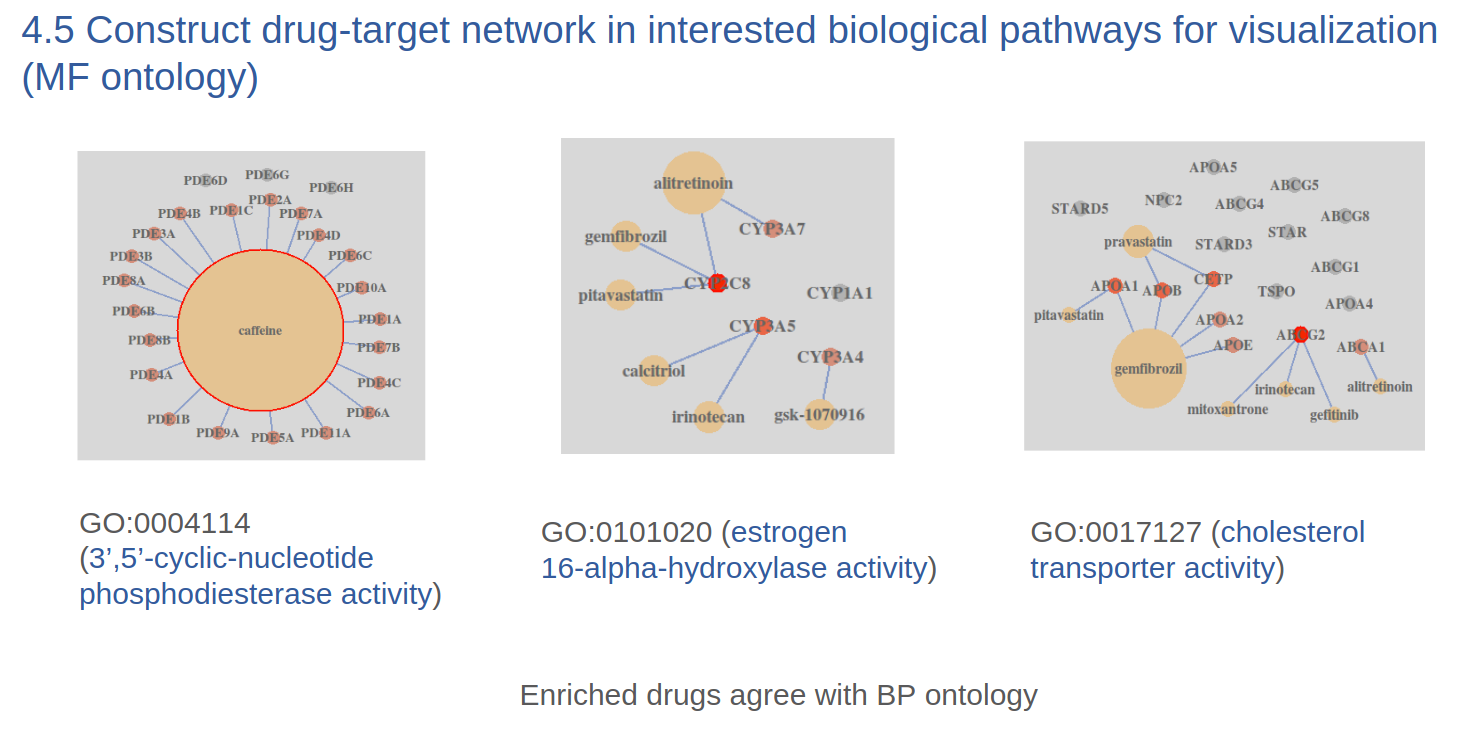
\includegraphics[width=12cm]{demo/images/dtnet_mf.png}
    \end{figure}
\end{frame}
%%%%%%%%%%%%%%%%%%%%%%%%%%%%%%%%% SLIDE %%%%%%%%%%%%%%%%%%%%%%%%%%%%%%%%%
\begin{frame}[fragile]{DSEA using MOA instead of GO/KEGG categories}
\vspace{-1.6cm}
\textcolor{blue}{Annotation resource:} \\
Drug MOA annotations in Touchstone database \\
\vspace{0.6cm}
\textcolor{blue}{Methods:} \\
hypergeometric test; GSEA \\
\vspace{0.6cm}
\textcolor{blue}{Query drug set:} \\ Top connected drugs in GESS result
\end{frame}
%%%%%%%%%%%%%%%%%%%%%%%%%%%%%%%%% SLIDE %%%%%%%%%%%%%%%%%%%%%%%%%%%%%%%%%
\begin{frame}[allowframebreaks]{References}
  \bibliography{demo}
  \bibliographystyle{elsart-harv.bst}
\end{frame}
%%%%%%%%%%%%%%%%%%%%%%%%%%%%%%%%% SLIDE %%%%%%%%%%%%%%%%%%%%%%%%%%%%%%%%%
\end{document}
